\documentclass[10pt,a4paper]{article}
\usepackage[T1]{fontenc}
\usepackage{lmodern}
\usepackage[margin=2.1cm]{geometry}
\usepackage{microtype}
\usepackage{booktabs}
\usepackage{graphicx}
\usepackage{amsmath,amssymb}
\usepackage{xcolor}
\usepackage{colortbl}
\usepackage{caption}
\usepackage{enumitem}
\usepackage{makecell}
\usepackage{float}
\usepackage{tabularx}
\usepackage[colorlinks=true,linkcolor=blue!50!black,citecolor=blue!50!black,urlcolor=blue!50!black]{hyperref}

\definecolor{best}{HTML}{E3F4EC}
\definecolor{grad}{HTML}{138A60}
\definecolor{note}{HTML}{F4F3EF}
\newcommand{\B}[1]{\textbf{#1}}
\newcommand{\cg}{\cellcolor{best}}
\setlist{itemsep=2pt,topsep=3pt}
\captionsetup{font=small,labelfont=bf}
\graphicspath{{figs/}{../figures/architectures/}}
\newcommand{\finding}[2]{\par\smallskip\noindent\colorbox{note}{\parbox{\dimexpr\linewidth-2\fboxsep}{\textbf{#1}\quad #2}}\par\smallskip}

\title{\textbf{V:N:M Sparsity for NEAT-Evolved Convolutional Networks}\\[4pt]
\large Evolving CNNs with CoDeepNEAT and compressing them with VENOM's V:N:M format\\
on CIFAR-10, CIFAR-100 and ImageNet-100}
\author{Final project report}
\date{October 2026}

\begin{document}
\maketitle

\begin{abstract}
\noindent
VENOM's V:N:M format extends the 2:4 sparsity of NVIDIA Sparse Tensor Cores to arbitrary sparsity levels.
It has so far been demonstrated on transformers.
This project asks whether it also works on convolutional networks, and specifically on networks found by neuro-evolution.
We evolve CNNs with CoDeepNEAT on CIFAR-10, CIFAR-100 and ImageNet-100.
We retrain the winners with a modern recipe and prune every convolution to V:2:M ($M\in\{4,8,16,32\}$, $V\in\{8,\dots,128\}$) with three criteria: magnitude, one-shot OBS and gradual OBS.
After a masked, distilled fine-tune we measure accuracy, stored size, and real inference time with VENOM's Spatha kernel.

\smallskip\noindent\textbf{Result.} V:N:M works on NEAT-evolved CNNs.
\begin{itemize}[leftmargin=*]
\item 2:4 ($3\times$ conv compression) is near-lossless on every well-trained model: median drop 0.3\,pt, at most 1.05\,pt.
\item The best evolved model (CIFAR-100, 76.5\% dense, 33.7\,MB) keeps 74.4\% at 2:8 (5.4\,MB) and 70.5\% at 2:16 (2.8\,MB).
\item At 2:32 (1.4\,MB, $25\times$) it keeps 63.7\% with gradual second-order pruning, 9.2\,pt more than magnitude pruning on average.
\item On CIFAR-10, the winner of an 80-generation search (11.1M parameters, 44.4\,MB) keeps its accuracy at 2:8 (86.5\% vs.\ 86.5\% for the identically fine-tuned dense model, 7.0\,MB) and loses 1\,pt at 2:16 (85.5\%, 3.5\,MB). An earlier 8-epoch recipe had made 2:16 look unusable (26\%).
\end{itemize}

\noindent Two new observations concern how evolved networks meet V:N:M.
\begin{itemize}[leftmargin=*]
\item The search space decides whether compression pays off. CoDeepNEAT's flatten+linear head leaves up to 77\% of the bytes unprunable. A residual-sum + global-average-pool space moves over 99\% of the bytes into prunable convolutions.
\item Evolved channel widths are irregular, so large $V$ forces row padding, which cuts 2:8 compression from $6.3\times$ to as low as $4.1\times$.
\end{itemize}

\noindent On speed, Spatha accelerates the conv GEMMs by $1.4$--$2.6\times$ at 2:8 and more at higher $M$.
A full forward pass, however, gains only $1.0$--$1.37\times$, because im2col and the non-conv layers are untouched.
V:N:M on CNNs is therefore, today, mainly a \emph{compression} result.
We also found that CoDeepNEAT's evaluator overstates accuracy by $n/(n{-}1)$ for $n$ test batches; affected numbers are corrected and the bug is fixed.
\end{abstract}

\tableofcontents
\newpage

%=====================================================================
\section{Introduction}
\subsection{Research question}
CoDeepNEAT~\cite{codeepneat} evolves CNN topologies by co-evolving small \emph{modules} and \emph{blueprints} that wire modules together.
The networks it finds are irregular: odd channel counts, large kernels, multi-way merges.
They are also dense and comparatively costly.
VENOM~\cite{venom} introduced the \emph{V:N:M} format, which keeps the hardware-friendly 2:4 pattern of Sparse Tensor Cores but reaches much higher sparsity through an extra vector (column) level.
Its Spatha kernel executes the resulting sparse matrix products.
The project question is:

\begin{quote}
\emph{Can V:N:M sparsity be applied to CNNs, and specifically to NEAT-evolved CNNs? What is the most accurate evolved model we can obtain at a given compression?}
\end{quote}

\noindent We say V:N:M ``works'' if three things hold:
\begin{enumerate}[label=(\alph*)]
\item accuracy after pruning and fine-tuning stays close to the dense model;
\item the packed format really reduces the stored model;
\item Spatha can execute the pruned convolutions, and we measure how fast.
\end{enumerate}

\subsection{Contributions}
\begin{enumerate}
\item \textbf{A V:N:M pipeline for CNNs:}
  \begin{itemize}
  \item conv$\to$GEMM layout, packing and byte accounting;
  \item three mask-selection criteria adapted to the V:N:M structure;
  \item masked fine-tuning with distillation;
  \item a Spatha-based convolution (im2col + sparse SpMM) verified against cuDNN on all 312 benchmark configurations.
  \end{itemize}
  We are not aware of prior V:N:M results on CNNs (Section~\ref{sec:lim}).
\item \textbf{Evidence that V:N:M works on NEAT-evolved CNNs} on three datasets, across 10 evolved models and the full $V\times M$ grid, including the winner of an 80-generation CIFAR-10 search.
\item \textbf{A V:N:M-friendly change to the CoDeepNEAT search space}: residual-sum aggregation and global average pooling. It raises the dense accuracy of the best evolved model by 4\,pt and turns $1.3\times$ whole-model compression into $24\times$.
\item \textbf{Findings specific to evolved networks} (Section~\ref{sec:novel}):
  \begin{itemize}
  \item the padding cost of irregular widths;
  \item the accuracy--speed tension in $V$;
  \item gradual second-order pruning as the decisive factor at high sparsity;
  \item why one-shot OBS gains vanish after fine-tuning;
  \item why evolved wide, large-kernel convs suit Spatha better than ResNet layers;
  \item two silent failure modes of the Spatha kernel;
  \item an accuracy bug in CoDeepNEAT's evaluator.
  \end{itemize}
\end{enumerate}

%=====================================================================
\section{Background}
\subsection{CoDeepNEAT}
CoDeepNEAT maintains two populations:
\begin{itemize}
\item \emph{modules}: small graphs of conv, BatchNorm, pooling and dropout layers;
\item \emph{blueprints}: graphs whose nodes are filled with a module drawn from a module species.
\end{itemize}
A blueprint plus its sampled modules forms a network, which is scored by validation accuracy after a short training run.
NEAT mutations add nodes and connections, and speciation protects new structure.
We use the PyTorch implementation by sash-a.
In the original code, branches are merged by channel concatenation and the classifier is \texttt{flatten}$\to$\texttt{linear}.

\subsection{V:N:M sparsity and Spatha}
A weight matrix $W\in\mathbb{R}^{R\times K}$ is tiled into blocks of $V$ rows by $M$ columns (Fig.~\ref{fig:format}).
\begin{itemize}
\item \textbf{Vector level:} in every block, 4 of the $M$ columns are kept, the same 4 for all $V$ rows.
\item \textbf{2:4 level:} inside those 4 columns, every row keeps $N{=}2$ values.
\end{itemize}
The density is $2/M$: 2:4, 2:8, 2:16 and 2:32 are 50\%, 75\%, 87.5\% and 93.75\% sparse, i.e.\ $2$, $4$, $8$ and $16\times$ fewer multiply-accumulates.

Spatha~\cite{venom} computes $Y=W_{\text{sparse}}X$. It gathers the kept columns of $X$ and feeds them to the 2:4 Sparse Tensor Core instruction (\texttt{mma.sp}).
Spatha is a matrix--matrix (SpMM) library and has no convolution kernel.

\subsection{Pruning criteria}
\begin{itemize}
\item \textbf{Magnitude:} keep the largest weights.
\item \textbf{Optimal Brain Surgeon (OBS)}~\cite{obs}: uses the curvature of the layer reconstruction loss, $H=\tfrac{2}{N}\sum xx^\top$ over the layer inputs $x$.
  \begin{itemize}
  \item The cost of removing $w_c$ is $w_c^2/[H^{-1}]_{cc}$; we rank with the squared form $w_c^2/[H^{-1}]_{cc}^2$ used by SparseGPT~\cite{sparsegpt}.
  \item The remaining weights are corrected by $\delta w=-\tfrac{w_c}{[H^{-1}]_{cc}}H^{-1}_{:,c}$.
  \end{itemize}
\item \textbf{VENOM's own criterion:} the \emph{gradual} second-order oBERT method~\cite{obert}.
\end{itemize}
N:M sparsity itself has been studied on CNNs~\cite{nm_nvidia,nm_zhou}, but only at 2:4-like densities that the hardware supports natively.

%=====================================================================
\section{How V:N:M was applied to CNNs}\label{sec:method}
This section describes the parts of the work that are specific to applying a GEMM-oriented sparse format to convolutions.

\subsection{Convolution as a GEMM}
\begin{figure}[H]
\centering
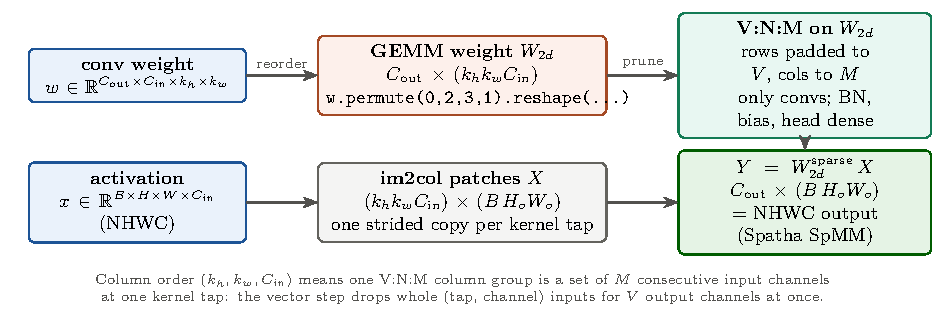
\includegraphics[width=\linewidth]{diag_conv_gemm.pdf}
\caption{Mapping a convolution onto the matrix that V:N:M prunes and Spatha multiplies.}
\label{fig:convgemm}
\end{figure}
A convolution with weights $w\in\mathbb{R}^{C_\text{out}\times C_\text{in}\times k_h\times k_w}$ is rewritten as
\[
W_{2d}=\texttt{w.permute(0,2,3,1).reshape(}C_\text{out},\,k_hk_wC_\text{in}\texttt{)},\qquad Y = W_{2d}\,X,
\]
where $X$ holds the im2col patches with the same $(k_h,k_w,C_\text{in})$ column order (Fig.~\ref{fig:convgemm}).
With this order, $C_\text{in}$ is the fastest-varying index, so an $M$-column group is $M$ consecutive input channels at one kernel tap.
The vector step of V:N:M therefore removes whole (tap, input-channel) pairs for a group of $V$ output channels.
CNNs tolerate this kind of structured removal well.
Only conv weights are pruned. BatchNorm, biases and the classifier stay dense in fp32.

\subsection{Format, packing and byte accounting}
\begin{figure}[H]
\centering
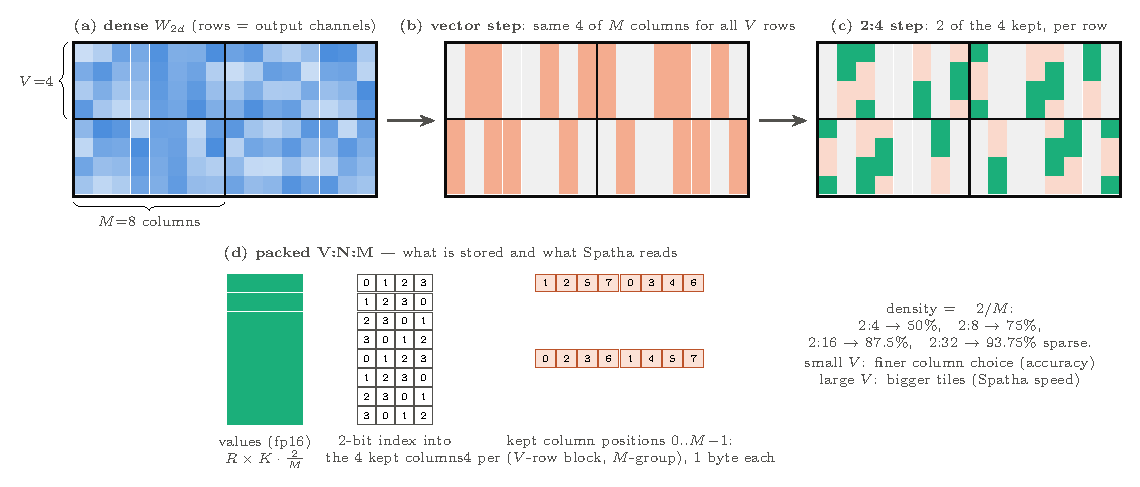
\includegraphics[width=\linewidth]{diag_vnm_format.pdf}
\caption{V:N:M on a toy $8\times16$ matrix with $V{=}4$, $M{=}8$ (2:8). (b)~The vector step keeps 4 columns per block. (c)~The 2:4 step keeps 2 of those per row. (d)~Stored form: dense fp16 values, a 2-bit index per value, and the kept column ids per block.}
\label{fig:format}
\end{figure}
\texttt{vnm/vnm\_pack.py} implements prune / pack / unpack.
\begin{itemize}
\item \textbf{Padding.} $W_{2d}$ is zero-padded to a multiple of $V$ rows and $M$ columns, and the packed tensors store the padded matrix.
\item \textbf{Stored bytes} (\texttt{packed\_nbytes\_tight}): 2 fp16 values per row per $M$-group, a 2-bit index per value, and, per $V$-row block and $M$-group, 4 kept-column positions $0..M{-}1$ at one byte each.
\item \textbf{Reported compression.} \emph{Conv compression} is fp32 dense conv bytes divided by packed conv bytes. \emph{Stored size} adds the dense fp32 non-conv parameters.
\item \textbf{Round trip.} \texttt{unpack(pack(W))} reproduces the pruned matrix exactly; this is asserted in every run.
\end{itemize}

Two consequences matter for evolved networks:
\begin{itemize}
\item \textbf{Metadata.} The column-id overhead shrinks as $V$ grows, because the ids are shared by more rows. On power-of-two layers, larger $V$ therefore \emph{raises} compression; ResNet-18 at 2:8 goes from $6.4\times$ at $V{=}8$ to $7.0\times$ at $V{=}128$.
\item \textbf{Row padding.} Evolved layers have channel counts such as 142, 171, 211 and 269. Padding them to a multiple of $V$ wastes storage and compute. bp482 at 2:8 drops from $6.3\times$ at $V{=}8$ to $4.1\times$ at $V{=}128$ (Section~\ref{sec:v}).
\end{itemize}

\subsection{Choosing the mask: three criteria}
\begin{figure}[H]
\centering
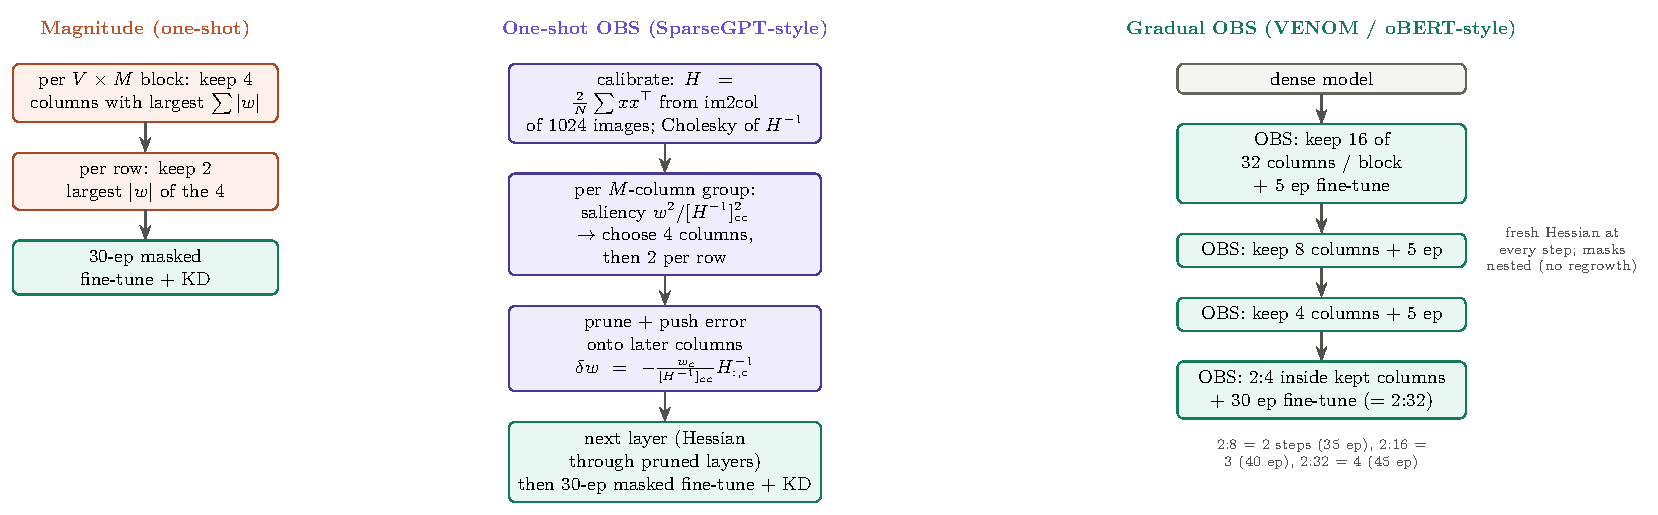
\includegraphics[width=\linewidth]{diag_pruning_methods.pdf}
\caption{The three mask-selection procedures. All end with the same masked, distilled fine-tune.}
\label{fig:methods}
\end{figure}
\paragraph{Magnitude (one-shot).} In each $V\times M$ block, keep the 4 columns with the largest $\sum|w|$ over the block's $V$ rows, then the 2 largest $|w|$ per row among them.

\paragraph{One-shot OBS, adapted to V:N:M} (\texttt{vnm/prune\_obs.py}). A SparseGPT-style layer-wise solver:
\begin{enumerate}
\item \textbf{Hessian.} $H=\tfrac{2}{N}\sum xx^\top$ over im2col patches of 1024 training images, with 1\% diagonal damping. We take the upper Cholesky factor of $H^{-1}$.
\item \textbf{Mask.} Columns are processed left to right in groups of $M$. At the start of each group, the V:N:M mask is chosen from the OBS saliency $w^2/[H^{-1}]_{cc}^2$: summed over the $V$ rows to choose 4 columns, then per row to choose 2.
\item \textbf{Compensation.} Each pruned column's error is pushed onto the columns not yet processed, with lazy updates in blocks of 128.
\item \textbf{Order.} Layers are pruned in module order. Each layer's Hessian is collected through the already-pruned layers before it.
\end{enumerate}

\paragraph{Gradual OBS (VENOM/oBERT-style)} (\texttt{vnm/prune\_gradual.py}). The target is reached in steps. Each step uses a fresh Hessian, an OBS pruning pass and a 5-epoch masked fine-tune:
\begin{itemize}
\item first, column (vector) pruning only, keeping $M/2\to M/4\to\dots\to4$ columns per block;
\item then a final 2:4 step inside the kept columns, followed by a 30-epoch fine-tune.
\end{itemize}
2:8, 2:16 and 2:32 take 2, 3 and 4 steps (35, 40 and 45 fine-tune epochs).
Masks are nested: weights removed in an earlier step have zero saliency and never come back.

\subsection{Recovering accuracy: masked fine-tune with distillation}
After pruning, the network is fine-tuned for 30 epochs:
\begin{itemize}
\item AdamW, lr $5\times10^{-4}$, wd 0.01, 1-epoch warm-up, then cosine;
\item knowledge distillation from the dense model ($\alpha{=}0.5$, $T{=}4$);
\item the mask is re-applied after every optimiser step, so the sparsity pattern is exactly preserved.
\end{itemize}

\subsection{Running pruned convolutions with Spatha}\label{sec:spathaconv}
\begin{figure}[H]
\centering
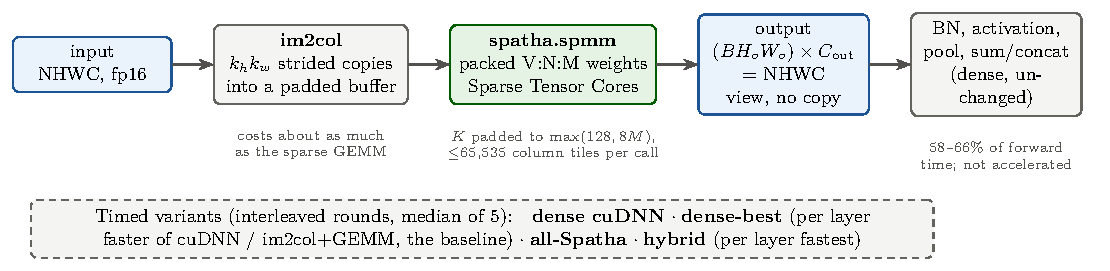
\includegraphics[width=\linewidth]{diag_spatha_conv.pdf}
\caption{Inference path of a V:N:M convolution (\texttt{SpathaConv2d} in \texttt{vnm/e2e\_bench.py}).}
\label{fig:spathaconv}
\end{figure}

\paragraph{Build.} We built Spatha from \texttt{UDC-GAC/venom} in a separate environment (PyTorch 1.13.1, CUDA 11.7) for sm\_86, which runs on our sm\_89 GPUs.
\begin{itemize}
\item $V$ equals Spatha's thread-block row tile, and the default build supports $V\in\{64,128\}$.
\item We added builds for $V{=}32$ and $V{=}256$.
\item $V\in\{8,16\}$ would need a kernel redesign (the warp tile is 32 rows). Those settings have accuracy and compression results but no timing.
\end{itemize}

\paragraph{Execution.} Every \texttt{Conv2d} of a pruned network is replaced by a \texttt{SpathaConv2d} (Fig.~\ref{fig:spathaconv}):
\begin{enumerate}
\item \textbf{im2col:} one strided copy per kernel tap writes the NHWC input straight into a padded $(k_hk_wC_\text{in})\times(BH_oW_o)$ buffer. This is $2\times$ faster than \texttt{F.unfold} plus a permute.
\item \textbf{SpMM:} \texttt{spatha.spmm} runs on the packed weights.
\item \textbf{Output:} the result, $(BH_oW_o)\times C_\text{out}$, is already NHWC and is used as a channels-last view without a copy.
\end{enumerate}

\paragraph{Correctness.} Spatha's own sparsifier can pick a different pattern among tied zeros, so we add $10^{-7}$ noise before conversion to reproduce our mask exactly.
Every one of the 312 end-to-end configurations was checked against cuDNN with the same masked weights on real test images: top-1 agreement $\ge99.2\%$, relative logit error $\le2.4\times10^{-3}$.

\paragraph{Two silent Spatha failures}, found and worked around:
\begin{itemize}
\item \textbf{(a) Out-of-bounds write at $M{=}32$.} When $K$ is an odd multiple of 128, the kernel writes out of bounds without an error, and cuBLAS/cuDNN calls made later crash. Fix: we pad $K$ to a multiple of $\max(128,8M)$.
\item \textbf{(b) Column-tile limit.} One call handles at most $65{,}535$ column tiles of 64 (about 4.2M columns). Beyond that it returns garbage without an error, so large inputs must be chunked; the ImageNet-100 check therefore uses 32 images.
\end{itemize}

%=====================================================================
\section{Experimental setup}
\subsection{Pipeline}
\begin{figure}[H]
\centering
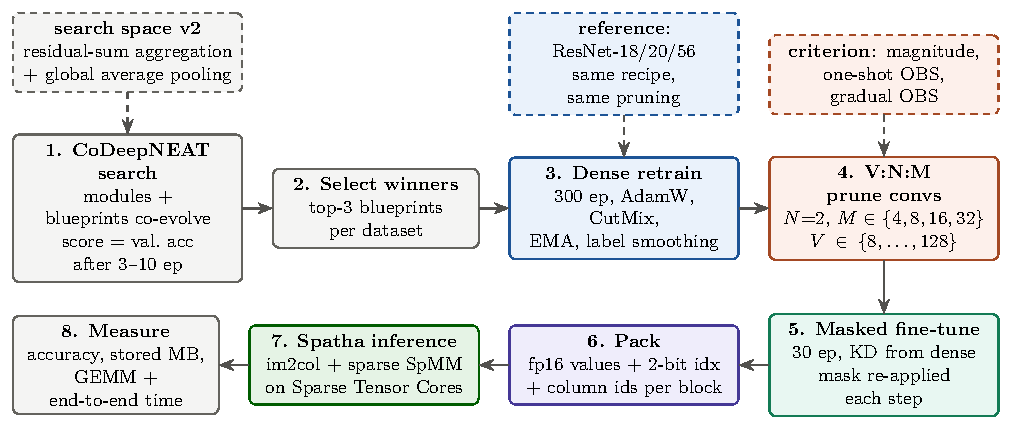
\includegraphics[width=\linewidth]{diag_pipeline.pdf}
\caption{End-to-end pipeline. V:N:M is applied post hoc to the winners of the search. Dashed boxes are the variations we added along the way.}
\label{fig:pipeline}
\end{figure}

\subsection{Hardware, software, data}
\begin{itemize}
\item \textbf{Hardware:} 3$\times$ NVIDIA RTX 6000 Ada (sm\_89, 48\,GB). They were \emph{shared}: other users' jobs often kept them at 100\% utilisation. Timings use interleaved rounds and medians to compensate.
\item \textbf{Software:}
  \begin{itemize}
  \item search, training and pruning: Python 3.13, PyTorch 2.6, bf16 autocast;
  \item Spatha: Python 3.10, PyTorch 1.13.1, CUDA 11.7.
  \end{itemize}
\item \textbf{Datasets:}
  \begin{itemize}
  \item CIFAR-10/100: 50k train, 10k test, $32^2$.
  \item ImageNet-100 (CMC split~\cite{cmc}): 126,689 train images; the 5,000 validation images are the test set. Images are cached at 144\,px with random $128^2$ crops for training, and resized to 146 with a $128^2$ centre crop for testing.
  \item Full ImageNet was not available on the machine.
  \end{itemize}
\item \textbf{Augmentation:}
  \begin{itemize}
  \item search: none (CoDeepNEAT's evolved augmentation was disabled);
  \item retraining and every V:N:M fine-tune: random crop and flip, plus CutMix in recipe v2.
  \end{itemize}
\end{itemize}

\subsection{A bug in CoDeepNEAT's evaluator, and how we corrected for it}\label{sec:evalbug}
CoDeepNEAT's \texttt{test\_nn} averages the per-batch accuracies and divides the sum by the index of the last batch, i.e.\ by $n-1$ for $n$ batches.
Every accuracy it reports is therefore inflated by $n/(n-1)$: $+1.3\%$ relative on a 10k test set at batch 128 ($n{=}79$), $+2.6\%$ at batch 256 ($n{=}40$) and $+2.5\%$ on ImageNet-100's 5,000 test images at batch 128.
We found it when CoDeepNEAT reported 87.68\% for a checkpoint that our own evaluator scores at 85.61\%; with the fix, CoDeepNEAT's evaluator gives 85.59\%.
\begin{itemize}
\item \textbf{Not affected:} everything evaluated by our own code (\texttt{vnm/recipe.py}): all retrained models, every 30-epoch V:N:M grid, OBS, gradual OBS, ResNets, ImageNet-100 after retraining, all timing. This is every main result.
\item \textbf{Affected:} numbers produced by CoDeepNEAT's evaluator: its 60-epoch full-train accuracies, the first V:N:M grids (CIFAR-10 small search, early CIFAR-100 and ImageNet-100 rows), and the search fitness. In this report the test-set numbers of the first group are \emph{corrected} by the factor $(n-1)/n$ (exact if every batch had the same accuracy; error ${\lesssim}0.1$\,pt) and marked $^{c}$. Search accuracies are left as logged (fitness is only used for ranking, which the factor does not change) and marked $^{s}$.
\item The evaluator in \texttt{final/} is fixed (every sample counts once), so re-running any script gives exact numbers.
\end{itemize}

\subsection{Searches}
\begin{table}[H]
\centering\small
\resizebox{\linewidth}{!}{%
\begin{tabular}{lccccc}
\toprule
 & CIFAR-10 & CIFAR-10 strong & CIFAR-100 & ImageNet-100 & CIFAR-100 res+GAP\\
\midrule
generations & 12 & \B{80} & 12 & 10 & 12\\
blueprint / module population & 20 / 50 & 25 / 80 & 20 / 50 & 10 / 20 & 20 / 50\\
evaluations $\times$ epochs per blueprint & $2\times3$ & \B{$4\times12$} & $2\times3$ & $2\times3$ & $2\times$\B{10}\\
batch / conv channels & 128 / 32--256 & 256 / 64--512 & 128 / 32--256 & 128 / 32--128 & 128 / 32--\B{384}\\
module species & 4 & 6 & 4 & 4 & 4\\
aggregation & concat & concat & concat & concat & \B{residual sum}\\
classifier head & flatten+linear & flatten+linear & flatten+linear & flatten+linear & \B{GAP+linear}\\
add-node / add-conn.\ rate (bp / module) & default & 0.16, 0.12 / 0.1 & default & default & 0.3 / 0.25\\
CoDeepNEAT full train of top 3 & 60 ep & 150 ep, fm 1 and 3 & 60 ep & 40 ep & 60 ep\\
wall-clock & 1.7\,h (3 GPUs) & about 2 days (2 GPUs) & 1.7\,h & 2.4\,h & 12.8\,h\\
\bottomrule
\end{tabular}}
\caption{Search configurations (\texttt{CoDeepNEAT/configuration/configs/*.json}; the strong CIFAR-10 search is \texttt{ada\_cifar10\_strong}). ``fm'' is CoDeepNEAT's feature multiplier, which rebuilds the same genotype with every channel count scaled so that the parameter count grows by that factor.}
\label{tab:search}
\end{table}

\subsection{Training recipes}
\begin{table}[H]
\centering\small
\begin{tabular}{@{}p{2.8cm}p{13.3cm}@{}}
\toprule
recipe v1 & AdamW, lr $2{\times}10^{-3}$, wd 0.05, 3-epoch warm-up + cosine, label smoothing 0.1, batch 128, crop + flip, bf16; 200 epochs (CIFAR-100), 120 epochs (ImageNet-100)\\
recipe v2 & v1 + \textbf{300 epochs}, CutMix ($p{=}0.5$, $\alpha{=}1$), EMA of weights (0.999; the better of live and EMA weights is kept)\\
V:N:M fine-tune & AdamW, lr $5{\times}10^{-4}$, wd 0.01, 30 epochs, KD ($\alpha{=}0.5$, $T{=}4$), mask re-applied after every step\\
\bottomrule
\end{tabular}
\caption{Recipes (\texttt{vnm/recipe.py}). The evolved architectures are kept unchanged; only their weights are retrained from scratch.}
\end{table}

\subsection{Experiment log}
Each experiment was motivated by the result of the previous one.
\begin{table}[H]
\centering\small
\renewcommand{\arraystretch}{1.1}
\begin{tabularx}{\linewidth}{@{}l>{\raggedright}p{4.6cm}X@{}}
\toprule
\# & experiment & outcome / why the next step\\
\midrule
E1 & Build Spatha for Ada; V:N:M pack/prune code; GEMM-level benchmark & Spatha correct within fp16 tolerance; $V\in\{32,64,128,256\}$ builds\\
E2 & Search on CIFAR-10, CIFAR-100, ImageNet-100 (orig.\ space) & winners found; CIFAR-100/IN-100 dense acc.\ only 42--49\% / 28--29\% (weak training loop)\\
E3 & First V:N:M grid (magnitude, 8-ep FT) & 2:4 lossless on CIFAR-10; higher $M$ unreliable on under-trained models $\to$ fix training\\
E4 & Retrain winners with recipe v1 (200 ep) & CIFAR-100 67\%, ImageNet-100 52--54\%\\
E5 & Full $V{\times}M$ grid, 30-ep KD FT (CIFAR-100, ImageNet-100) & graceful degradation, $V{=}8$ best\\
E6 & Recipe v2 (300 ep, CutMix, EMA) + grid & CIFAR-100 evolved 72.4\%\\
E7 & ResNet-18/20/56 from scratch, same recipe + grid & ResNets lead by about 6\,pt; evolved heads not compressible $\to$ change search space\\
E8 & Residual-sum + GAP search, retrain top 6, grid on top 3 & 76.5\% dense; convs hold $>$99\% of bytes\\
E9 & One-shot OBS (V:N:M-aware) & large zero-shot gain, small gain after FT\\
E10 & Gradual OBS (VENOM-style) & +9.2\,pt at 2:32 over magnitude\\
E11 & Spatha GEMM timing on every pruned conv; $V$-scan on synthetic shapes & 1.4--2.6$\times$ at 2:8\\
E12 & End-to-end Spatha inference, 12 models $\times$ 3 $V$ $\times$ 4 $M$ $\times$ 2 batch sizes & 1.0--1.27$\times$ whole-network\\
E13 & Strong CIFAR-10 search (80 generations), CoDeepNEAT full train at fm 1 and 3; 8-epoch magnitude recover on the winner bp1485 & 2:4 recovers to dense, 2:8 loses about 6\,pt, 2:16 fails; found the evaluator bug\\
E14 & Our pipeline on bp1485: 30-ep KD grid, dense control, gradual OBS, Spatha timing & see Section~\ref{sec:c10}\\
\bottomrule
\end{tabularx}
\caption{Experiments in the order they were run.}
\end{table}

%=====================================================================
\section{Results}
\subsection{The searches and the evolved architectures}
\begin{figure}[H]
\centering
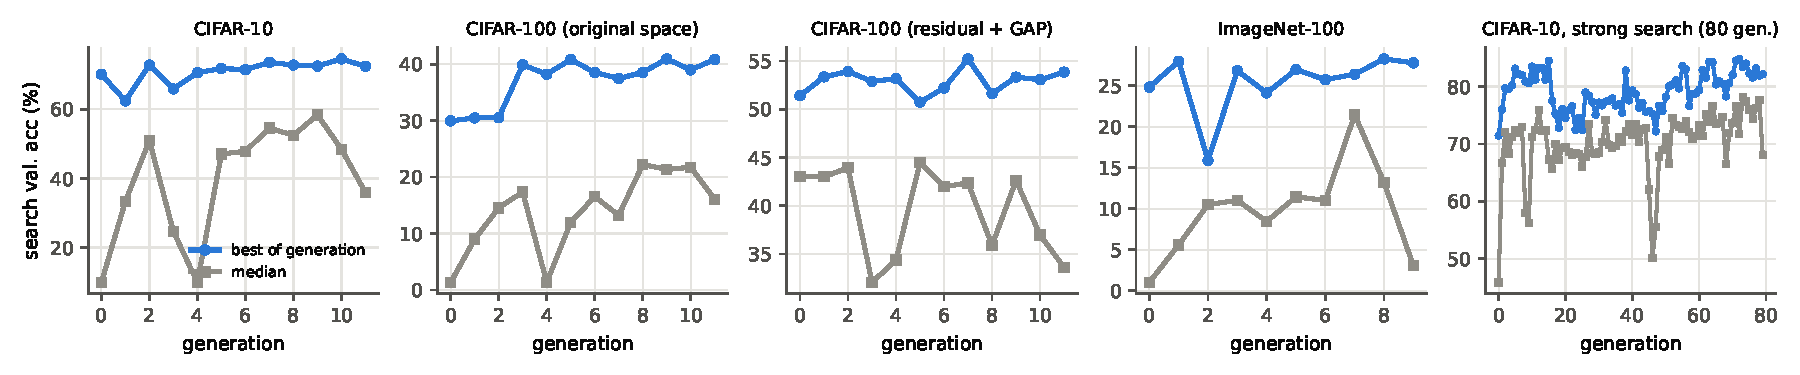
\includegraphics[width=\linewidth]{search_progress.pdf}
\caption{Search fitness (validation accuracy) per generation, as logged by CoDeepNEAT ($^{s}$, slightly inflated; Section~\ref{sec:evalbug}). First four panels: our searches (40 evaluations per generation; 20 on ImageNet-100). Right: the 80-generation strong CIFAR-10 search (best and median blueprint of each generation). The best of a generation rises by 3--14\,pt over a run; the median fluctuates widely because new structure is evaluated after only 3--12 epochs.}
\label{fig:search}
\end{figure}

\begin{table}[H]
\centering\small
\resizebox{\linewidth}{!}{%
\begin{tabular}{llrrlll}
\toprule
search & model & params & convs & kernels & conv widths & bytes in convs\\
\midrule
CIFAR-100 res+GAP & bp493 & 8.42M & 10 & $1,3,5,7$ & 142--342 & 99.7\%\\
CIFAR-100 res+GAP & bp482 & 2.51M & 6 & $3,5$ & 142--342 & 99.2\%\\
CIFAR-100 res+GAP & bp741 & 4.33M & 5 & $3,5,7$ & 148--291 & 99.6\%\\
CIFAR-100 orig.\ & bp430 / bp427 & 3.62M / 3.27M & 10 & $1,5$ & 44--457 & 60\% / 66\%\\
CIFAR-100 orig.\ & bp499 & 5.49M & 7 & $1,5$ & 44--457 & \B{23\%}\\
\bottomrule
\end{tabular}}
\caption{Evolved CIFAR-100 winners. All are shallow (5--10 convs) and wide, with large kernels and irregular channel counts. The original space puts most of the bytes into the dense flatten+linear head.}
\label{tab:arch}
\end{table}

\finding{Observation.}{Scoring candidates after only 3--10 epochs favours shallow, wide, large-kernel networks that converge quickly. This has two consequences: dense accuracy is capped below hand-designed deep networks, but the convolutions are large GEMMs that suit Spatha (Section~\ref{sec:speed}).}

\subsection{Dense accuracy}
\begin{figure}[H]
\centering
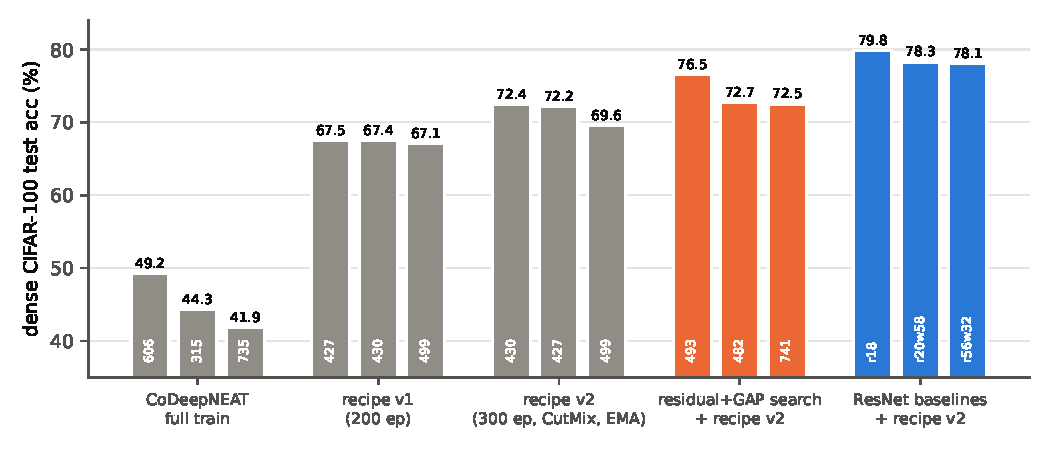
\includegraphics[width=0.86\linewidth]{dense_progress.pdf}
\caption{Dense CIFAR-100 test accuracy of the top 3 models at each stage. Better training lifts the same evolved architectures from at most 50\% to 72\%. The residual+GAP search adds 4\,pt more at the top.}
\label{fig:dense}
\end{figure}

\begin{table}[H]
\centering\small
\resizebox{\linewidth}{!}{%
\begin{tabular}{llrrr}
\toprule
dataset & model & params & search acc.$^{s}$ & final dense acc.\\
\midrule
CIFAR-10 & evolved bp495 / bp671 / bp546 (small search) & 1.91M / 0.57M / 2.84M & -- & 80.60 / 79.73 / 78.26$^{c}$\\
CIFAR-10 & evolved bp1485, fm 3 (strong search) & 11.11M & 84.5$^{s}$ & \B{85.61}\\
CIFAR-100 & evolved bp430 / bp427 / bp499 (recipe v2) & 3.62M / 3.27M / 5.49M & 38.5 / 38.3 / 37.5 & 72.39 / 72.17 / 69.57\\
CIFAR-100 & evolved res+GAP bp493 / bp482 / bp741 (v2) & 8.42M / 2.51M / 4.33M & 55.2 / 54.2 / 53.9 & \B{76.50} / 72.69 / 72.47\\
ImageNet-100 & evolved bp207 / bp182 / bp230 (v1, 120 ep) & 2.77M / 3.05M / 0.47M & 25.7 / 26.0 / 28.3 & 53.68 / 52.36 / 52.28\\
\midrule
CIFAR-100 & ResNet-18 / ResNet-20 (w58) / ResNet-56 (w32) & 11.22M / 3.58M / 3.42M & -- & 79.83 / 78.26 / 78.08\\
\bottomrule
\end{tabular}}
\caption{Dense models that were pruned. CIFAR-10 models use CoDeepNEAT's own full-train weights (60 epochs; 150 epochs at fm 3 for bp1485). $^{c}$\,corrected for the evaluator bug; $^{s}$\,search fitness as logged (Section~\ref{sec:evalbug}).}
\label{tab:dense}
\end{table}

\subsection{CIFAR-100: accuracy versus compression}\label{sec:c100}
\begin{table}[H]
\centering\small
\setlength{\tabcolsep}{4pt}
\resizebox{\linewidth}{!}{%
\begin{tabular}{lllrr|rrrr}
\toprule
family & criterion & model & params & dense & 2:4 & 2:8 & 2:16 & 2:32\\
 & & & & & ($3.1\times$) & ($6.3\times$) & ($12.6\times$) & ($25\times$)\\
\midrule
evolved res+GAP & magnitude & bp493 & 8.42M & \cg76.50 & \cg76.26 & 74.01 & 70.06 & 57.23\\
 & OBS one-shot & bp493 & & & -- & 73.92 & 69.23 & 57.98\\
 & \textcolor{grad}{OBS gradual} & bp493 & & & -- & \cg\B{74.40} & \cg\B{70.50} & \cg\B{63.72}\\
evolved res+GAP & magnitude & bp741 & 4.33M & 72.47 & 72.20 & 70.15 & 66.60 & 57.05\\
 & OBS one-shot & bp741 & & & -- & 70.45 & 66.43 & 57.11\\
 & \textcolor{grad}{OBS gradual} & bp741 & & & -- & \B{70.92} & \B{68.09} & \B{61.78}\\
evolved res+GAP & magnitude & bp482 & 2.51M & 72.69 & 72.44 & 69.60 & 62.14 & 42.37\\
 & OBS one-shot & bp482 & & & -- & 69.94 & 62.75 & 47.23\\
 & \textcolor{grad}{OBS gradual} & bp482 & & & -- & \B{70.24} & \B{64.33} & \B{55.37}\\
\midrule
evolved (orig.) & magnitude & bp430 & 3.62M & 72.39 & 71.34 & 68.40 & 62.40 & 49.79\\
evolved (orig.) & magnitude & bp427 & 3.27M & 72.17 & 71.50 & 68.61 & 62.35 & 50.50\\
evolved (orig.) & magnitude & bp499 & 5.49M & 69.57 & 69.29 & 66.84 & 63.42 & 56.53\\
\bottomrule
\end{tabular}}
\caption{CIFAR-100, evolved models (recipe v2), 30-epoch KD fine-tune after pruning (35--45 epochs for gradual OBS). Cells: test accuracy (\%), best over $V\in\{8,\dots,128\}$; the best $V$ is almost always 8. Shaded: best evolved result per column. Compression is conv-only and nearly identical across models at a given $M$.}
\label{tab:c100}
\end{table}

\begin{figure}[H]
\centering
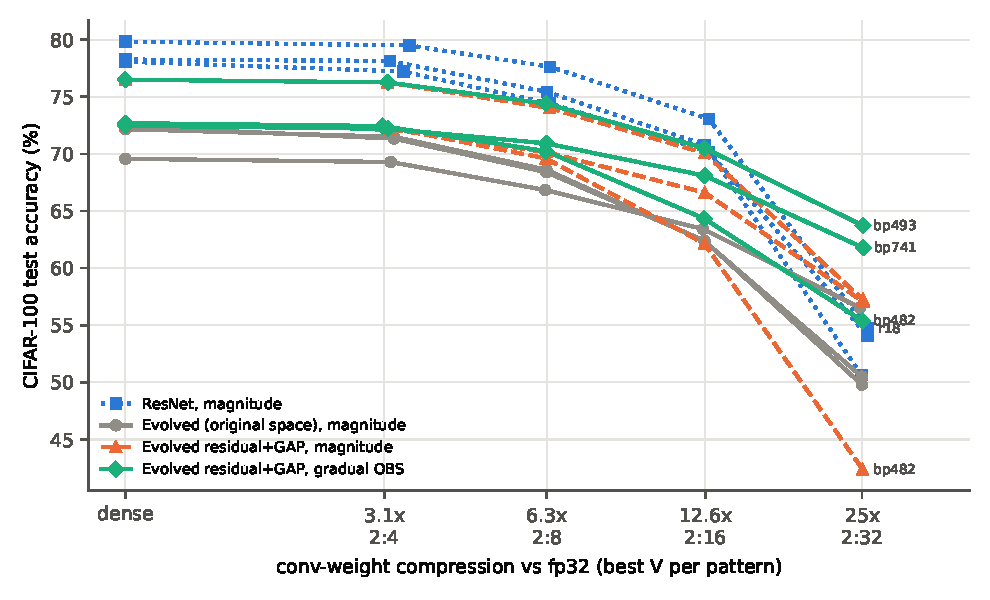
\includegraphics[width=0.86\linewidth]{c100_acc_vs_comp.pdf}
\caption{CIFAR-100 accuracy against conv compression (best $V$ per pattern). Gradual OBS (aqua) lifts the evolved residual models above every magnitude-pruned curve at $25\times$, including the ResNets (blue, dotted).}
\label{fig:c100}
\end{figure}

\finding{V:N:M works on evolved CNNs.}{2:4 costs 0.24--1.05\,pt. 2:8 costs 2.3--4\,pt with magnitude pruning and 1.6--2.5\,pt with gradual OBS. 2:16 costs 5.9--10.6\,pt with magnitude pruning and 4.4--8.4\,pt with gradual OBS, for 8$\times$ fewer MACs. The degradation is smooth, with no cliff until 2:32 under magnitude pruning.}

\subsection{Stored size: why the search space mattered}
\begin{figure}[H]
\centering
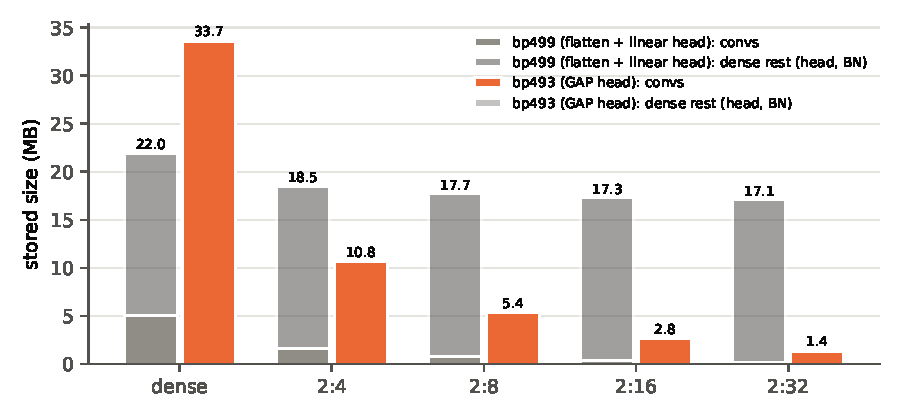
\includegraphics[width=0.78\linewidth]{model_size.pdf}
\caption{Stored size at $V{=}8$. bp499 (original space) keeps a 17\,MB dense flatten+linear head, so even 2:32 only shrinks it $1.3\times$. bp493 (GAP head) shrinks 33.7\,MB $\to$ 10.8 / 5.4 / 2.8 / 1.4\,MB.}
\label{fig:size}
\end{figure}
In the original search space, conv compression does not become model compression.
After we added residual-sum aggregation and a GAP head, over 99\% of the bytes sit in convolutions and the whole model shrinks by the conv ratio.
Figure~\ref{fig:pareto} shows every CIFAR-100 configuration we trained on the size--accuracy plane.
Below about 1\,MB, the frontier consists of gradual-OBS evolved models.

\begin{figure}[H]
\centering
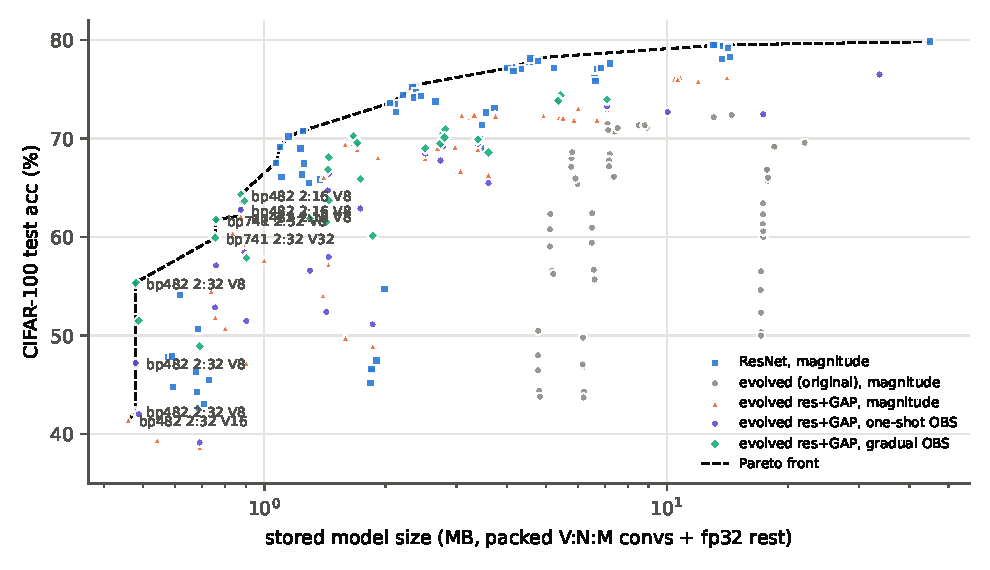
\includegraphics[width=0.86\linewidth]{pareto_size.pdf}
\caption{All CIFAR-100 runs (every model, $V$, $M$ and criterion): accuracy against stored size. The dashed line is the Pareto front. Above about 2\,MB, the size-matched ResNets dominate. At the smallest sizes, the gradual-OBS evolved models form the front.}
\label{fig:pareto}
\end{figure}

\subsection{Pruning criterion: magnitude vs.\ one-shot OBS vs.\ gradual OBS}\label{sec:crit}
\begin{table}[H]
\centering\small
\begin{tabular}{lrrrc}
\toprule
pattern & gradual $-$ magnitude & gradual $-$ one-shot & one-shot $-$ magnitude & gradual beats magnitude\\
\midrule
2:8 & +0.62 & +0.37 & +0.26 & 8 / 9\\
2:16 & +2.48 & +2.78 & $-$0.30 & 9 / 9\\
2:32 & \B{+9.18} & +7.71 & +1.48 & 9 / 9\\
\bottomrule
\end{tabular}
\caption{Mean accuracy difference after fine-tuning (points), over 3 evolved residual models $\times$ $V\in\{8,32,128\}$. Per-run values are in Appendix~\ref{app:obs}.}
\label{tab:obs}
\end{table}

\begin{figure}[H]
\centering
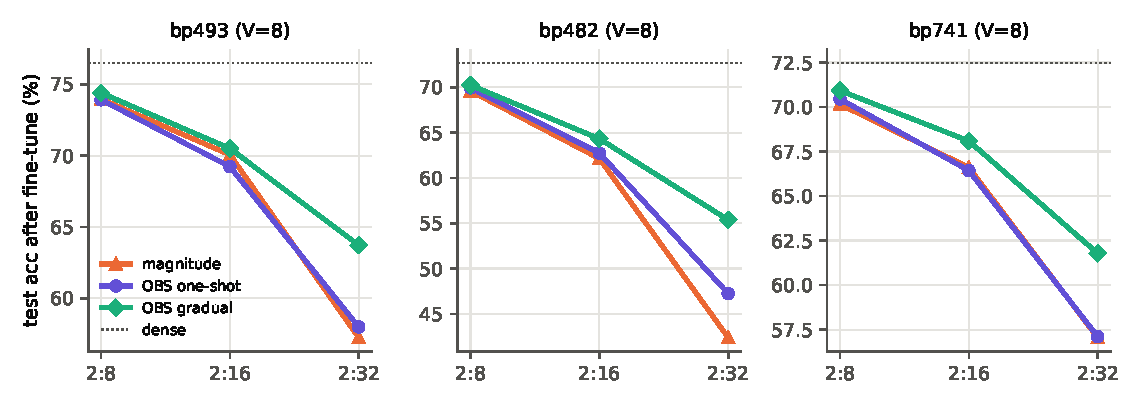
\includegraphics[width=\linewidth]{method_compare.pdf}
\caption{Fine-tuned accuracy of the three criteria at $V{=}8$. Dotted line: dense model.}
\end{figure}

\begin{figure}[H]
\centering
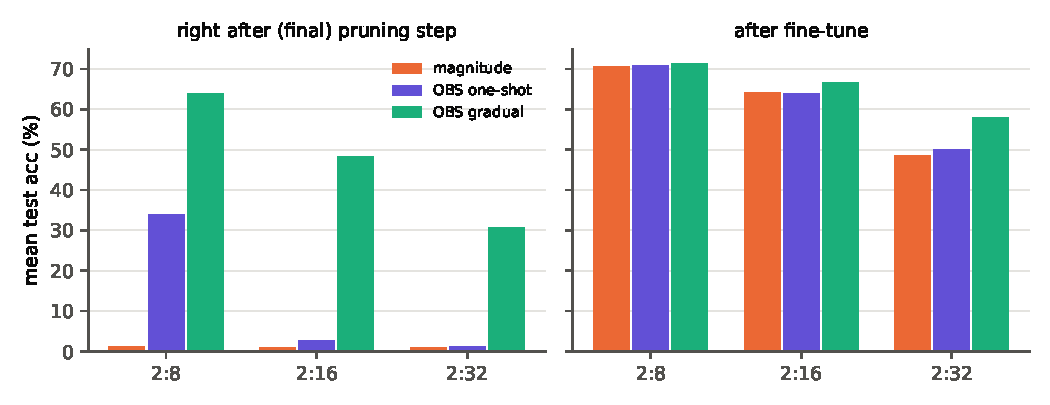
\includegraphics[width=0.86\linewidth]{zero_vs_ft.pdf}
\caption{Left: accuracy right after the (final) pruning step. Right: after fine-tuning. One-shot OBS leaves a far better starting point than magnitude pruning: at 2:8, 22--49\% instead of about 1\%. Fine-tuning erases that advantage, while the gradual gain persists and grows with sparsity.}
\label{fig:zero}
\end{figure}

\begin{figure}[H]
\centering
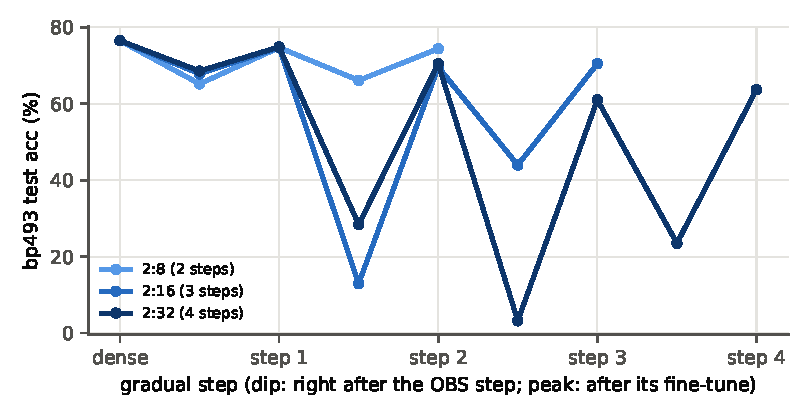
\includegraphics[width=0.66\linewidth]{gradual_trajectory.pdf}
\caption{Gradual OBS on bp493 ($V{=}8$). The first column step (half the columns removed) costs only about 2\,pt after 5 epochs. Most of the damage happens in the last column steps, and the final 2:4 step plus its 30-epoch fine-tune \emph{recovers} accuracy (2:32: 61.0 $\to$ 63.7\%).}
\label{fig:traj}
\end{figure}

\finding{At high sparsity, the criterion matters more than the architecture.}{With magnitude pruning, 2:32 collapses to 42--57\% for every family. Gradual OBS adds 5--13\,pt and gives the best 2:32 result in the study, 63.7\% at $25\times$. The gain comes from moving into the sparse subspace \emph{gradually} and re-estimating curvature along the way, which is why VENOM uses gradual oBERT. A good one-shot starting point is not enough.}

\subsection{Effect of $V$ and the padding cost of evolved widths}\label{sec:v}
\begin{figure}[H]
\centering
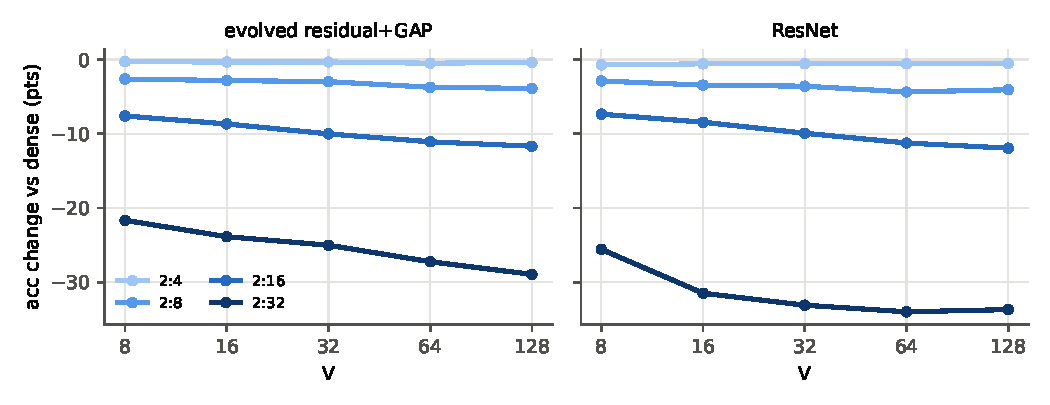
\includegraphics[width=0.86\linewidth]{effect_of_v.pdf}
\caption{Mean accuracy change against dense as a function of $V$ (magnitude pruning, 3 models each). Smaller $V$ is better at every $M$, and the effect grows with $M$. At 2:4, $V$ hardly matters (spread at most 0.8\,pt).}
\label{fig:v}
\end{figure}
Smaller $V$ means the 4 kept columns are chosen for fewer rows, so the mask is closer to unstructured 2:$M$.
The accuracy cost of $V{=}128$ over $V{=}8$ is 1--3\,pt at 2:8 and 3--5\,pt at 2:16.
$V$ also changes \emph{compression}, and here evolved networks behave differently from hand-designed ones (Fig.~\ref{fig:pad}).

\begin{figure}[H]
\centering
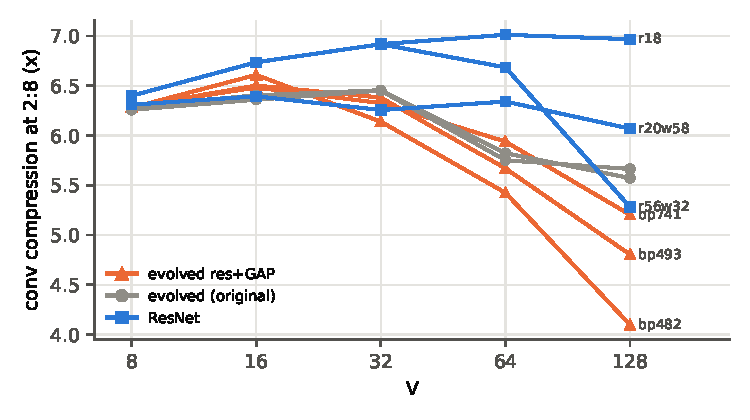
\includegraphics[width=0.62\linewidth]{padding_vs_v.pdf}
\caption{Conv compression at 2:8 as a function of $V$.
\textbf{ResNets:} power-of-two widths, so larger $V$ amortises the column ids and compression rises up to $V{=}64$--128.
\textbf{Evolved networks:} irregular widths (142, 171, 211, 269, \dots) are padded up to $V$ rows, so compression falls from $6.3\times$ to $4.1$--$5.7\times$ at $V{=}128$.}
\label{fig:pad}
\end{figure}

\subsection{CIFAR-10: the strong search and its winner}\label{sec:c10}
Our own CIFAR-10 search (12 generations, 3-epoch evaluations) was short.
A second, much longer CIFAR-10 search was run on the same machine (\texttt{ada\_cifar10\_strong}, Table~\ref{tab:search}): 80 generations, 4 evaluations of 12 epochs per blueprint, wider channel range, followed by CoDeepNEAT's 150-epoch full train of the top 3 at feature multiplier 1 and 3.
We take its winner through our whole pipeline.

\paragraph{Search and winner.}
The best-of-generation fitness rises from 71\% to about 85\% over the 80 generations (Fig.~\ref{fig:search}, right).
The winner, blueprint 1485, was only third in the evolution ranking but first after full training (Table~\ref{tab:c10ft}).
Its three blueprint nodes all use module 1463 (species 19): a narrowing $3{\times}3$ conv with BN, dropout 0.1 and LeakyReLU, then a widening $3{\times}3$ conv with $3{\times}3$/stride-3 max-pooling, dropout 0.37 and ReLU6.
A skip from the stem module is concatenated with a side branch (Fig.~\ref{fig:bp1485}).
At feature multiplier 3 the network has six convs with 329 / 624 channels, a 1248-channel concatenation, and 11.1M parameters.
Because the max-pools shrink the map to $4{\times}4$, the flatten+linear head is tiny: \B{99.9\% of the bytes are convolutions}, so this model needed no change of search space to be compressible.

\begin{figure}[H]
\centering
\begin{minipage}{0.55\linewidth}\centering\includegraphics[width=\linewidth]{ada_cifar10_strong_bp1485_phenotype.png}\end{minipage}\hfill
\begin{minipage}{0.4\linewidth}\centering\includegraphics[width=\linewidth]{ada_cifar10_strong_bp1485_blueprint_genome.png}\end{minipage}
\caption{bp1485 drawn by CoDeepNEAT's own visualisers. Left: phenotype at feature multiplier 3 (yellow: module layers; violet: concatenation). Right: genotype; all three blueprint nodes point at species 19 / module 1463.}
\label{fig:bp1485}
\end{figure}

\begin{table}[H]
\centering\small
\begin{tabular}{lcrr}
\toprule
model (fm 3) & evolution rank & CoDeepNEAT full train (150 ep)$^{c}$ & saved checkpoint, exact\\
\midrule
bp6826 & 1 & 85.45 & --\\
bp6724 & 2 & 84.42 & --\\
\B{bp1485} & 3 & 85.98 (peak) & \B{85.61}\\
\bottomrule
\end{tabular}
\caption{Full training of the top 3. $^{c}$\,CoDeepNEAT reported 87.64 / 86.58 / 88.18\%; corrected for the evaluator bug (Section~\ref{sec:evalbug}). The pruning experiments start from the saved checkpoint, which our evaluator scores at 85.61\%.}
\label{tab:c10ft}
\end{table}

\paragraph{V:N:M results.}
Table~\ref{tab:c10} compares three ways of recovering accuracy after pruning bp1485.
The first is the original study's recipe: magnitude pruning at $V{=}8$, then 8 epochs of Adam (lr $10^{-4}$) with the mask re-applied, no augmentation and no distillation.
Re-run with the fixed evaluator it reproduces the reported numbers once corrected (2:4 86.0\%, 2:8 79.8\%, 2:16 26.4\%; reported 88.29 / 81.72 / 23.65\% under the bug).
The second is our 30-epoch recipe (crop + flip, distillation from the dense model).
Because that recipe also trains the dense model further, we add a \B{dense control}: the unpruned model fine-tuned with the identical 30-epoch recipe reaches 86.45\%, which is the fair reference.

\begin{table}[H]
\centering\small
\setlength{\tabcolsep}{5pt}
\resizebox{\linewidth}{!}{%
\begin{tabular}{ll|rrrr}
\toprule
recovery after pruning & $V$ & 2:4 & 2:8 & 2:16 & 2:32\\
 & & ($3.2\times$, 14.0\,MB) & ($6.3\times$, 7.0\,MB) & ($12.6\times$, 3.5\,MB) & ($25\times$, 1.8\,MB)\\
\midrule
none (zero-shot) & 8 & 41.11 & 16.53 & 10.97 & 10.00\\
8-ep Adam, no aug., no KD (original study) & 8 & 86.01 & 79.78 & 26.36 & --\\
30-ep KD fine-tune, magnitude & 8 & 86.30 & \B{86.52} & \B{85.48} & 79.11\\
30-ep KD fine-tune, magnitude & 32 & \B{86.35} & 86.36 & 85.02 & 80.52\\
gradual OBS & 8 & -- & -- & 84.42 & \B{81.55}\\
gradual OBS & 32 & -- & -- & 83.33 & 80.35\\
\midrule
\multicolumn{6}{l}{dense checkpoint 85.61\,\% (44.4\,MB); \B{dense control}, same 30-ep fine-tune without pruning: \B{86.45}\,\%}\\
\bottomrule
\end{tabular}}
\caption{CIFAR-10, bp1485 (11.1M parameters, fm 3). Test accuracy (\%), all with the fixed evaluator. Sizes are conv bytes packed at $V{=}8$ ($V{=}32$ is slightly smaller: 13.5 / 6.7 / 3.4 / 1.7\,MB), plus 44\,KB of dense non-conv parameters.}
\label{tab:c10}
\end{table}

\begin{itemize}
\item \textbf{The weak recipe, not V:N:M, limited the original study.} With our fine-tune, 2:8 matches the dense control (86.52 vs 86.45\%) and 2:16 is within 1\,pt of it (85.48\%) at $12.6\times$ compression, where the 8-epoch recipe gave 26\%.
\item \textbf{The best CIFAR-10 result:} a 44.4\,MB evolved CNN stored in 3.5\,MB at 85.5\% (2:16), or in 7.0\,MB with no loss (2:8).
\item \textbf{$V$ hardly matters on this network} (within 0.5\,pt at 2:4--2:16, and $V{=}32$ is better at 2:32), unlike on the CIFAR-100 models. Its layers are wide (329--1248 channels), so the vector constraint costs little and row padding is small.
\item \textbf{Gradual OBS} helps only at the highest sparsity: at 2:32 and $V{=}8$ it gives 81.55\% against 79.11\% for magnitude pruning ($+2.4$\,pt), the best 2:32 result on this network. At 2:16, and at $V{=}32$, it is 0.2--1.7\,pt \emph{below} magnitude pruning. This is the opposite of CIFAR-100, where gradual OBS added 9.2\,pt at 2:32: on this wide network with a well-tuned fine-tune, magnitude pruning already leaves little to recover.
\end{itemize}

\subsection{ImageNet-100}
\begin{table}[H]
\centering\small
\begin{tabular}{lrr|rrrr}
\toprule
model & params & dense & 2:4 & 2:8 & 2:16 & 2:32\\
\midrule
bp207 & 2.77M & 53.68 & \B{54.30} & 53.28 & 48.00 & 38.70\\
bp182 & 3.05M & 52.36 & 51.84 & 50.24 & 47.48 & 41.60\\
bp230 & 0.47M & 52.28 & 51.96 & 49.26 & 45.38 & 40.12\\
\bottomrule
\end{tabular}
\caption{ImageNet-100, retrained 120 epochs, magnitude pruning with a 30-epoch KD fine-tune, best over $V$. bp207 at 2:4 \emph{exceeds} its dense accuracy: the distilled fine-tune acts as extra training.}
\label{tab:other}
\end{table}
\begin{figure}[H]
\centering
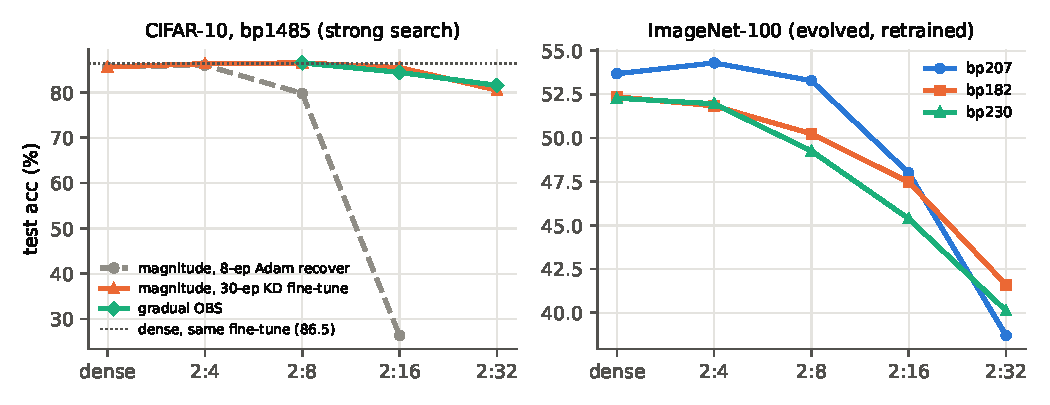
\includegraphics[width=0.86\linewidth]{other_datasets.pdf}
\caption{Left: CIFAR-10 winner bp1485 under the three recovery schemes (best $V$; dashed: the 8-epoch recipe of the original study; dotted: the dense model with the same 30-epoch fine-tune). Right: ImageNet-100, which degrades gracefully to 38.7--41.6\% at 2:32.}
\end{figure}
The small CIFAR-10 search of our own (bp495 / bp671 / bp546, CoDeepNEAT weights, 8-epoch fine-tune) is in Appendix~\ref{app:early}.

\subsection{Speed}\label{sec:speed}
\paragraph{GEMM level.}
Each pruned conv is timed as an im2col GEMM, Spatha against a dense fp16 GEMM of the same shape, excluding im2col itself.
\begin{figure}[H]
\centering
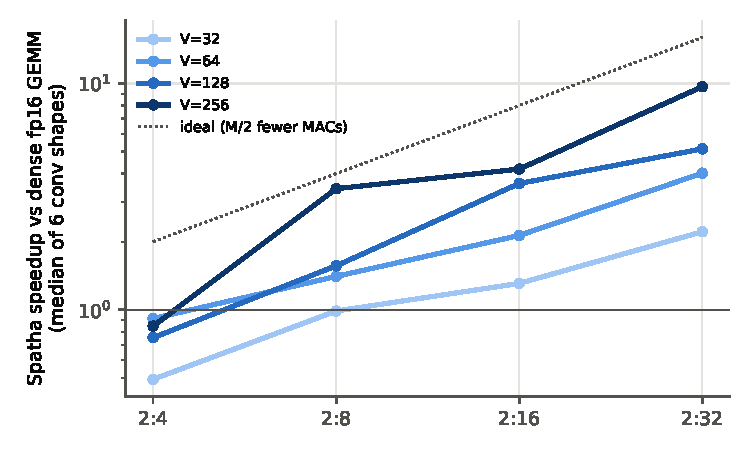
\includegraphics[width=0.6\linewidth]{vscan.pdf}
\caption{Spatha SpMM speedup on six typical conv GEMM shapes (batch 128). The speedup grows with $V$ and $M$. At 2:4 Spatha is \emph{slower} than dense for most $V$.}
\label{fig:vscan}
\end{figure}

\begin{table}[H]
\centering\small
\setlength{\tabcolsep}{4pt}
\resizebox{\linewidth}{!}{%
\begin{tabular}{l|rrrr|rrrr|rrrr}
\toprule
 & \multicolumn{4}{c|}{$V=32$} & \multicolumn{4}{c|}{$V=64$} & \multicolumn{4}{c}{$V=128$}\\
model & 2:4 & 2:8 & 2:16 & 2:32 & 2:4 & 2:8 & 2:16 & 2:32 & 2:4 & 2:8 & 2:16 & 2:32\\
\midrule
bp493 (res) & 0.95 & 1.43 & 2.12 & 3.84 & 1.16 & 1.77 & 2.81 & 5.44 & 1.10 & 1.83 & 3.66 & 7.88\\
bp741 (res) & 0.93 & 1.56 & 2.32 & 3.66 & 1.18 & 2.11 & 3.14 & 4.75 & 1.22 & 2.06 & 3.55 & 5.84\\
bp482 (res) & 0.89 & 1.77 & 5.37 & 14.0$^\dagger$ & 1.40 & 1.98 & 5.95 & 16.9$^\dagger$ & 1.66 & 2.57 & 7.35 & 29.6$^\dagger$\\
bp430 (orig.) & 0.85 & 1.68 & 3.11 & 5.68 & 1.19 & 2.16 & 3.67 & 9.66 & 1.26 & 2.50 & 5.37 & 19.1$^\dagger$\\
r18 & 0.65 & 1.23 & 13.3$^\dagger$ & 23.1$^\dagger$ & 0.86 & 4.12 & 15.5$^\dagger$ & 25.8$^\dagger$ & 0.95 & 2.23 & 14.8$^\dagger$ & 25.4$^\dagger$\\
r56w32 & 0.08 & 0.93 & 1.47 & 1.93 & 0.07 & 1.06 & 1.65 & 1.65 & 0.08 & 0.24 & 1.27 & 1.65\\
ImageNet-100 bp207 & -- & -- & -- & -- & 0.98 & 1.49 & 2.39 & 3.64 & 0.85 & 1.54 & 2.51 & 3.44\\
\bottomrule
\end{tabular}}
\caption{Summed conv-GEMM speedup (batch 128). $^\dagger$\,Above the ideal $M/2$ reduction, so inflated by an unstable dense baseline on the shared GPUs: read as ``large''. Narrow ResNet-56 (32-channel layers padded to $V$) is launch-bound and does not speed up.}
\label{tab:speed}
\end{table}

\paragraph{End to end.}
Every conv of the network runs through \texttt{SpathaConv2d}, and the whole forward pass is timed.
Speedups are against \emph{dense-best}: per layer, the faster of cuDNN and the same im2col path with a dense GEMM. This isolates what sparsity adds.
\begin{figure}[H]
\centering
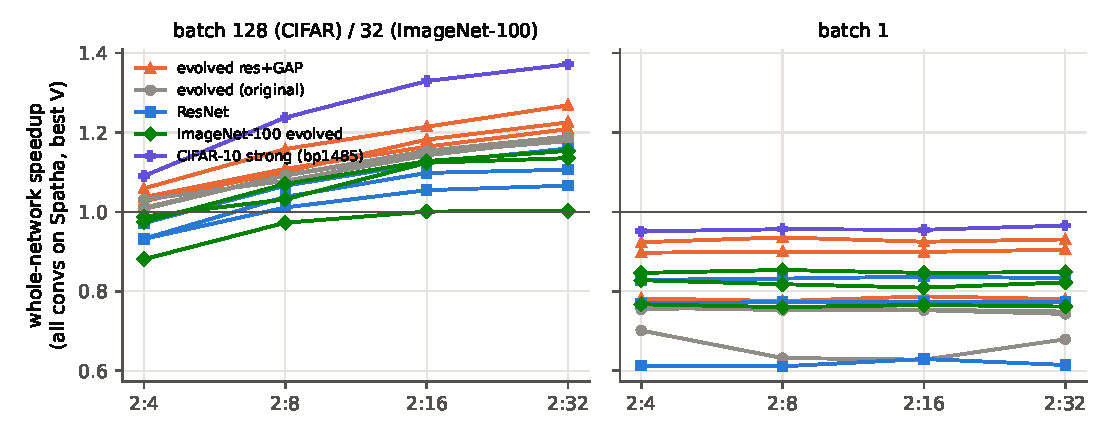
\includegraphics[width=\linewidth]{e2e_speedup.pdf}
\caption{Whole-network inference speedup with every conv on Spatha (best $V$). At large batch the gain grows with $M$ but stays below $1.4\times$; the CIFAR-10 winner bp1485 (widest convs) gains most. At batch 1 Spatha is slower (overhead-bound).}
\label{fig:e2e}
\end{figure}

\begin{table}[H]
\centering\small
\resizebox{\linewidth}{!}{%
\begin{tabular}{llr|rrrr|rrrr}
\toprule
 & & dense-best & \multicolumn{4}{c|}{all-Spatha} & \multicolumn{4}{c}{hybrid (per-layer fastest)}\\
dataset & model & ms & 2:4 & 2:8 & 2:16 & 2:32 & 2:4 & 2:8 & 2:16 & 2:32\\
\midrule
CIFAR-100 & bp493 (res) & 24.3 & 1.03 & 1.10 & 1.18 & 1.23 & 1.03 & 1.09 & 1.17 & 1.21\\
CIFAR-100 & bp741 (res) & 16.4 & 1.06 & 1.16 & 1.21 & 1.27 & 1.07 & 1.16 & 1.22 & 1.27\\
CIFAR-100 & bp482 (res) & 6.3 & 1.04 & 1.11 & 1.16 & 1.21 & 1.05 & 1.11 & 1.17 & 1.21\\
CIFAR-100 & bp430 (orig.) & 7.4 & 1.01 & 1.09 & 1.15 & 1.18 & 1.07 & 1.16 & 1.21 & 1.23\\
CIFAR-100 & bp427 (orig.) & 7.3 & 1.03 & 1.08 & 1.14 & 1.18 & 1.07 & 1.14 & 1.22 & 1.26\\
CIFAR-100 & bp499 (orig.) & 7.2 & 1.01 & 1.09 & 1.15 & 1.19 & 1.10 & 1.15 & 1.23 & 1.24\\
CIFAR-100 & r18 & 17.7 & 0.97 & 1.07 & 1.12 & 1.16 & 1.00 & 1.07 & 1.12 & 1.14\\
CIFAR-100 & r20w58 & 21.7 & 0.93 & 1.04 & 1.10 & 1.11 & 1.00 & 1.03 & 1.09 & 1.09\\
CIFAR-100 & r56w32 & 29.6 & 0.93 & 1.01 & 1.05 & 1.07 & 0.99 & 1.02 & 1.05 & 1.07\\
CIFAR-10 & bp1485 (strong) & 22.6 & 1.09 & 1.24 & 1.33 & \B{1.37} & 1.09 & 1.25 & 1.33 & \B{1.37}\\
ImageNet-100 & bp207 & 14.4 & 0.97 & 1.07 & 1.13 & 1.15 & 1.01 & 1.08 & 1.14 & 1.17\\
ImageNet-100 & bp182 & 12.5 & 0.99 & 1.03 & 1.12 & 1.14 & 1.03 & 1.07 & 1.13 & 1.18\\
ImageNet-100 & bp230 & 1.6 & 0.88 & 0.97 & 1.00 & 1.00 & 1.01 & 1.01 & 1.01 & 1.01\\
\midrule
\multicolumn{3}{l|}{all models, batch 1} & \multicolumn{4}{c|}{0.50--0.94} & \multicolumn{4}{c}{0.85--1.03}\\
\bottomrule
\end{tabular}}
\caption{End-to-end speedup of a full forward pass (best over $V\in\{32,64,128\}$) relative to dense-best, at batch 128 (CIFAR) or 32 (ImageNet-100). Medians of 5 interleaved rounds; median round-to-round spread 2\%. All 312 runs: \texttt{results/end\_to\_end/e2e.csv}. bp1485 was timed later, while our own training jobs shared the GPUs.}
\label{tab:e2e}
\end{table}

\begin{figure}[H]
\centering
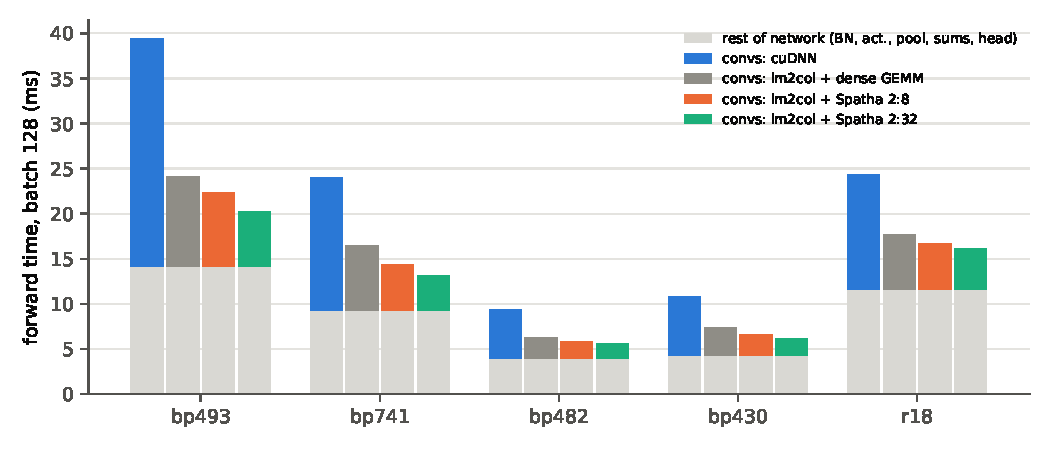
\includegraphics[width=0.86\linewidth]{time_breakdown.pdf}
\caption{Where the time goes ($V{=}128$, batch 128). The grey base is everything that is not a convolution; on top is the conv time of each implementation. Convolutions are only 34--42\% of the dense-best forward pass. Within them, im2col costs about as much as the sparse GEMM: for bp493 at 2:32 the GEMM is about $8\times$ faster, but im2col + Spatha is only $1.6\times$ faster than im2col + dense GEMM.}
\label{fig:breakdown}
\end{figure}

\finding{Speed is limited by Amdahl's law, applied twice.}{Convolutions are under half of the forward time (60\% at most, for the CIFAR-10 winner), and within each convolution the im2col copy is as expensive as the sparse GEMM. A 4--8$\times$ GEMM speedup therefore becomes a 1.1--1.37$\times$ network speedup. Evolved models gain more than ResNets (1.27--1.37$\times$ vs.\ 1.16$\times$) because their wide, large-kernel convs make the GEMM a larger share of the conv.}

\subsection{Comparison with hand-designed ResNets (brief)}
As a sanity check, we trained CIFAR ResNets from scratch with the identical recipe and pruned them identically. Figure~\ref{fig:rn} summarises the comparison.
\begin{itemize}
\item \textbf{Dense accuracy:} ResNet-20/56 are 1.6--1.8\,pt more accurate than the best evolved model at under half its size; ResNet-18 is 3.3\,pt more accurate and larger.
\item \textbf{2:4 to 2:16:} under the same magnitude pruning, the \emph{drop} from dense is the same for both families. Evolved topologies are not harder to sparsify.
\item \textbf{2:32:} gradual OBS on the evolved models (63.7\%) beats every magnitude-pruned ResNet (best 54.7\%). OBS was not run on the ResNets, so this compares criteria as much as architectures.
\end{itemize}
\begin{figure}[H]
\centering
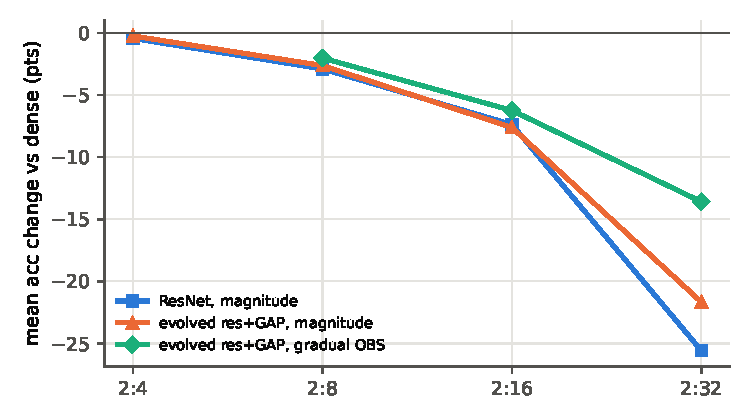
\includegraphics[width=0.56\linewidth]{resnet_vs_evolved.pdf}
\caption{Mean accuracy change against dense (best $V$, 3 models per family).}
\label{fig:rn}
\end{figure}

%=====================================================================
\section{Was V:N:M useful?}
\textbf{Yes, as compression; only modestly as acceleration.}
\begin{table}[H]
\centering\small
\resizebox{\linewidth}{!}{%
\begin{tabular}{llrrrrr}
\toprule
goal & configuration (bp493, CIFAR-100) & acc.\ & conv comp.\ & stored & conv GEMM speedup & end-to-end (bs 128)\\
\midrule
dense reference & -- & 76.50 & $1\times$ & 33.7\,MB & -- & --\\
near-lossless & $V{=}8$, 2:4, magnitude & 76.26 & $3.1\times$ & 10.8\,MB & -- ($V{=}8$) & --\\
balanced, Spatha-runnable & $V{=}32$, 2:8, magnitude & 74.01 & $6.4\times$ & 5.4\,MB & $1.43\times$ & $1.08\times$\\
best 2:8 & $V{=}8$, 2:8, gradual OBS & 74.40 & $6.3\times$ & 5.4\,MB & -- & --\\
high compression & $V{=}8$, 2:16, gradual OBS & 70.50 & $12.6\times$ & 2.8\,MB & -- & --\\
max compression & $V{=}8$, 2:32, gradual OBS & \B{63.72} & $25.1\times$ & \B{1.4\,MB} & -- & --\\
max comp., Spatha-runnable & $V{=}32$, 2:32, gradual OBS & 61.50 & $25.5\times$ & $\approx$1.4\,MB & $3.84\times$ & $1.19\times$\\
\bottomrule
\end{tabular}}
\caption{Recommended operating points for the best evolved CIFAR-100 model. Speedups are measured on the same $(V,M)$ pattern; kernel time depends only on the pattern, not on the weight values.}
\label{tab:ops}
\end{table}

\begin{table}[H]
\centering\small
\resizebox{\linewidth}{!}{%
\begin{tabular}{llrrrr}
\toprule
goal & configuration (bp1485, CIFAR-10) & acc.\ & conv comp.\ & stored & end-to-end (bs 128)\\
\midrule
dense reference & 30-ep fine-tuned, no pruning (control) & 86.45 & $1\times$ & 44.4\,MB & --\\
lossless & $V{=}8$, 2:8, magnitude, 30-ep KD & \B{86.52} & $6.3\times$ & 7.0\,MB & --\\
lossless, Spatha-runnable & $V{=}32$, 2:8, magnitude, 30-ep KD & 86.36 & $6.6\times$ & 6.7\,MB & $1.11\times$\\
high compression & $V{=}8$, 2:16, magnitude, 30-ep KD & 85.48 & $12.6\times$ & \B{3.5\,MB} & --\\
high comp., Spatha-runnable & $V{=}32$, 2:16, magnitude, 30-ep KD & 85.02 & $13.2\times$ & 3.4\,MB & $1.25\times$\\
max compression & $V{=}32$, 2:32, magnitude, 30-ep KD & 80.52 & $26.3\times$ & 1.7\,MB & \B{1.30$\times$}\\
max compression, best accuracy & $V{=}8$, 2:32, gradual OBS & 81.55 & $25.3\times$ & 1.8\,MB & --\\
\bottomrule
\end{tabular}}
\caption{Operating points for the CIFAR-10 winner (dense checkpoint 85.61\%, 44.4\,MB fp32). End-to-end speedup with every conv on Spatha, against the fastest dense implementation of each layer.}
\label{tab:ops10}
\end{table}
\begin{itemize}
\item \textbf{Storage.} On CIFAR-100 a 33.7\,MB evolved CNN becomes 5.4\,MB with 2.1\,pt loss, or 1.4\,MB with 12.8\,pt loss; this is only possible because the residual+GAP search space puts the parameters into convolutions. On CIFAR-10 a 44.4\,MB evolved CNN becomes 7.0\,MB with no loss and 3.5\,MB with 1\,pt loss.
\item \textbf{Executability.} Every pruned network runs on Sparse Tensor Cores through Spatha and matches cuDNN to fp16 precision.
\item \textbf{Speed.} The sparse GEMMs are 1.4--8$\times$ faster, but whole networks are only 1.1--1.37$\times$ faster at large batch and not faster at batch 1.
\end{itemize}

%=====================================================================
\section{Novel findings}\label{sec:novel}
\begin{enumerate}
\item \textbf{V:N:M transfers to CNNs through the $(k_h,k_w,C_\text{in})$ im2col layout.}
  \begin{itemize}
  \item Across 15 well-trained CNNs on three datasets, 2:4 loses a median 0.3\,pt.
  \item 2:8 loses 2--4\,pt on CIFAR-100 and 0.4--3\,pt on ImageNet-100, and nothing on the wide CIFAR-10 winner, which loses 1\,pt at 2:16.
  \item In this layout, the vector step removes (tap, input-channel) pairs for groups of output channels, and convolutions tolerate that well.
  \end{itemize}
\item \textbf{The NAS search space decides whether V:N:M pays off.}
  \begin{itemize}
  \item The default CoDeepNEAT space leaves 34--77\% of the bytes in an unprunable flatten+linear head, which caps whole-model compression at about $1.3$--$2\times$.
  \item Residual-sum aggregation plus GAP moves 99\%+ of the bytes into convs, giving $24\times$ whole-model compression. It also raised dense accuracy by 4\,pt.
  \item Searching for sparse deployment needs a sparsity-friendly space, not just a better pruner.
  \end{itemize}
\item \textbf{Irregular evolved widths clash with large $V$.}
  \begin{itemize}
  \item Row padding to a multiple of $V$ cuts 2:8 compression from $6.3\times$ to $4.1$--$5.7\times$ at $V{=}128$ on evolved models.
  \item On power-of-two ResNet widths, larger $V$ instead \emph{improves} compression, to $7.0\times$, through shared column ids.
  \item A V:N:M-aware search should constrain channel counts to multiples of $V$.
  \end{itemize}
\item \textbf{Accuracy and speed favour opposite $V$.} Accuracy is best at $V{=}8$. Spatha exists only for $V\ge32$ and is fastest at $V{=}128$. The cost of $V{=}128$ is 1--3\,pt at 2:8 and 3--5\,pt at 2:16.
\item \textbf{Gradual second-order pruning is what makes high V:N:M sparsity usable on the CIFAR-100 models.}
  \begin{itemize}
  \item It adds 9.2\,pt on average at 2:32 and wins 26 of 27 comparisons.
  \item One-shot OBS improves zero-shot accuracy by up to 48\,pt, but that gain mostly disappears after fine-tuning. Zero-shot accuracy is therefore a poor proxy for the final result.
  \item In the gradual schedule, removing the first half of the columns (vector-only sparsity) costs only about 2\,pt, and the final 2:4 step with a long fine-tune recovers accuracy.
  \item How much it helps depends on the network: on the wide CIFAR-10 winner it adds only 2.4\,pt at 2:32 and nothing below that.
  \end{itemize}
\item \textbf{Evolved CNNs are more Spatha-friendly than deep thin ResNets.}
  \begin{itemize}
  \item Short-budget evolution produces shallow, wide, large-kernel networks ($5\times5$ and $7\times7$, 142--342 channels; up to 1248 on CIFAR-10).
  \item Their GEMMs are large, so they gain the most end to end: up to $1.27\times$ on CIFAR-100 and $1.37\times$ for the CIFAR-10 winner (2:32, $V{=}128$), whose convs are 60\% of its forward time, against 34--42\% for the other models.
  \item ResNet-56 with 32-channel layers does not speed up at all.
  \end{itemize}
\item \textbf{Two silent failure modes of Spatha.}
  \begin{itemize}
  \item At $M{=}32$, $K$ must be padded to a multiple of 256, otherwise there is an out-of-bounds write.
  \item One call is limited to 65,535 column tiles, beyond which it returns garbage.
  \end{itemize}
  Neither is documented, and both corrupt results or later kernels without any error.
\item \textbf{The recovery recipe decides what looks feasible.} On the same CIFAR-10 checkpoint, an 8-epoch Adam recover without augmentation or distillation gives 26\% at 2:16; our 30-epoch distilled fine-tune with crop and flip gives 85.5\%, 1\,pt below a dense model fine-tuned the same way. Because such a fine-tune also improves the dense model (85.6 $\to$ 86.5\%), V:N:M results should be compared against an equally fine-tuned dense control.
\item \textbf{CoDeepNEAT's evaluator overstates accuracy by $n/(n{-}1)$} for $n$ test batches (it divides the summed batch accuracies by the last batch index): $+1.3\%$ relative at batch 128 on CIFAR, $+2.6\%$ at 256. Published or reported CoDeepNEAT accuracies computed with it should be read with this in mind. It is fixed in our copy.
\item \textbf{Training dominates search for the final accuracy.} The same evolved architectures went from at most 50\% to 72.4\% on CIFAR-100 (and from 28.9\% to 52.3\% on ImageNet-100) by retraining alone. Pruning studies on under-trained evolved models (Appendix~\ref{app:early}) understate how much V:N:M can retain.
\end{enumerate}

%=====================================================================
\section{Limitations}\label{sec:lim}
\begin{itemize}
\item \textbf{Single seed, test-set selection.} Each cell is one run, and ``best over $V$'' and the top models were picked on the test set. Differences under about 0.5\,pt are not significant.
\item \textbf{Unequal fine-tune budget.} Gradual OBS had 35--45 epochs against 30.
  \begin{itemize}
  \item One-shot OBS and magnitude pruning, at equal budget, are within 0.3\,pt of each other at 2:8 and 2:16, so we believe the extra epochs are not the main cause of the 2:32 gain.
  \item The definitive control, gradual \emph{magnitude} pruning on the same schedule, was not run.
  \end{itemize}
\item \textbf{OBS was not applied to the ResNets.}
\item \textbf{Timing.}
  \begin{itemize}
  \item GPUs were shared and fully loaded.
  \item Execution was PyTorch 1.13 eager mode, without operator fusion or CUDA graphs.
  \item $V{=}8/16$ settings cannot be timed.
  \item GEMM-level numbers marked $^\dagger$ exceed the theoretical bound.
  \end{itemize}
\item \textbf{Search.} Our own searches were short (10--12 generations); only the strong CIFAR-10 search ran 80 generations. No search used augmentation or a VENOM-aware fitness.
\item \textbf{CIFAR-10 winner.} Only one model (bp1485) went through the full pipeline; its dense weights come from CoDeepNEAT's training without augmentation, which is why the dense control is needed.
\item \textbf{Literature.} We found no prior V:N:M results on CNNs (VENOM evaluates transformers), but we did not do a systematic search.
\end{itemize}

\section{Future work}
\begin{itemize}
\item Gradual magnitude pruning as a control; gradual OBS on the ResNets; multiple seeds with a validation split.
\item A VENOM-aware search:
  \begin{itemize}
  \item score candidates \emph{after} V:N:M pruning, or add size/latency as an objective;
  \item restrict channel counts to multiples of $V$;
  \item use longer evaluations so deeper networks can win.
  \end{itemize}
\item An implicit-GEMM Spatha convolution (no im2col), fused BN/activation epilogues, and $V{=}8/16$ kernels, followed by new end-to-end measurements.
\item Full ImageNet.
\end{itemize}

\section{Conclusion}
V:N:M sparsity applies cleanly to CNNs, including the irregular networks found by CoDeepNEAT, provided two things hold:
\begin{itemize}
\item the search space puts the parameters into convolutions (residual sum + GAP);
\item high sparsity is reached gradually with second-order pruning.
\end{itemize}
The best evolved CIFAR-100 model goes from 33.7\,MB to 5.4\,MB at 74.4\% (2:8) and to 1.4\,MB at 63.7\% (2:32). The CIFAR-10 winner of an 80-generation search goes from 44.4\,MB to 7.0\,MB with no loss and to 3.5\,MB at 85.5\% (2:16), once it is fine-tuned properly. Every pruned network runs on Sparse Tensor Cores.
The remaining gap is inference speed: turning large sparse-GEMM speedups into network speedups needs a sparse convolution kernel that avoids im2col.

%=====================================================================
\clearpage
\appendix
\section{Per-run comparison of pruning criteria}\label{app:obs}
\begin{table}[H]
\centering\small
\begin{tabular}{rrl|rrr|rr}
\toprule
bp & $V$ & $M$ & magnitude & OBS one-shot & OBS gradual & grad.$-$mag. & grad.$-$1-shot\\
\midrule
482 & 8 & 2:8 & 69.60 & 69.94 & 70.24 & +0.64 & +0.30\\
482 & 8 & 2:16 & 62.14 & 62.75 & 64.33 & +2.19 & +1.58\\
482 & 8 & 2:32 & 42.37 & 47.23 & 55.37 & +13.00 & +8.14\\
482 & 32 & 2:8 & 68.94 & 69.33 & 69.58 & +0.64 & +0.25\\
482 & 32 & 2:16 & 59.02 & 58.44 & 63.65 & +4.63 & +5.21\\
482 & 32 & 2:32 & 41.95 & 42.03 & 51.49 & +9.54 & +9.46\\
482 & 128 & 2:8 & 67.99 & 68.47 & 68.99 & +1.00 & +0.52\\
482 & 128 & 2:16 & 56.95 & 56.59 & 61.89 & +4.94 & +5.30\\
482 & 128 & 2:32 & 38.67 & 39.14 & 48.89 & +10.22 & +9.75\\
\midrule
493 & 8 & 2:8 & 73.97 & 73.92 & 74.40 & +0.43 & +0.48\\
493 & 8 & 2:16 & 70.06 & 69.23 & 70.50 & +0.44 & +1.27\\
493 & 8 & 2:32 & 57.23 & 57.98 & 63.72 & +6.49 & +5.74\\
493 & 32 & 2:8 & 74.01 & 73.75 & 73.83 & $-$0.18 & +0.08\\
493 & 32 & 2:16 & 67.69 & 67.76 & 69.49 & +1.80 & +1.73\\
493 & 32 & 2:32 & 52.79 & 52.38 & 61.50 & +8.71 & +9.12\\
493 & 128 & 2:8 & 72.97 & 73.26 & 73.95 & +0.98 & +0.69\\
493 & 128 & 2:16 & 66.34 & 65.46 & 68.57 & +2.23 & +3.11\\
493 & 128 & 2:32 & 48.94 & 51.13 & 60.14 & +11.20 & +9.01\\
\midrule
741 & 8 & 2:8 & 70.15 & 70.45 & 70.92 & +0.77 & +0.47\\
741 & 8 & 2:16 & 66.60 & 66.43 & 68.09 & +1.49 & +1.66\\
741 & 8 & 2:32 & 57.05 & 57.11 & 61.78 & +4.73 & +4.67\\
741 & 32 & 2:8 & 69.71 & 70.03 & 70.10 & +0.39 & +0.07\\
741 & 32 & 2:16 & 64.85 & 64.72 & 66.86 & +2.01 & +2.14\\
741 & 32 & 2:32 & 51.85 & 52.85 & 59.91 & +8.06 & +7.06\\
741 & 128 & 2:8 & 68.96 & 69.46 & 69.90 & +0.94 & +0.44\\
741 & 128 & 2:16 & 63.29 & 62.89 & 65.90 & +2.61 & +3.01\\
741 & 128 & 2:32 & 47.20 & 51.48 & 57.89 & +10.69 & +6.41\\
\bottomrule
\end{tabular}
\caption{Every run of the criterion comparison (CIFAR-100, evolved residual+GAP models).}
\end{table}

\section{Accuracy by $V$ (CIFAR-100, magnitude)}
\begin{table}[H]
\centering\small
\begin{tabular}{l|rrrrr|rrrrr}
\toprule
 & \multicolumn{5}{c|}{2:4} & \multicolumn{5}{c}{2:8}\\
model & $V$=8 & 16 & 32 & 64 & 128 & 8 & 16 & 32 & 64 & 128\\
\midrule
bp493 & 76.26 & 76.09 & 76.03 & 75.84 & 76.21 & 73.97 & 73.89 & 74.01 & 73.09 & 72.97\\
bp741 & 72.20 & 72.15 & 72.14 & 71.93 & 71.91 & 70.15 & 69.80 & 69.71 & 69.18 & 68.96\\
bp482 & 72.24 & 72.36 & 72.44 & 72.34 & 72.35 & 69.60 & 69.43 & 68.94 & 68.11 & 67.99\\
bp430 & 71.18 & 71.30 & 71.34 & 71.34 & 71.10 & 68.40 & 67.77 & 67.17 & 65.97 & 66.10\\
bp427 & 71.07 & 70.86 & 71.50 & 70.70 & 71.07 & 68.61 & 67.99 & 67.12 & 65.93 & 65.39\\
bp499 & 69.24 & 69.29 & 69.18 & 69.25 & 69.26 & 66.84 & 66.83 & 66.84 & 65.71 & 66.02\\
r18 & 79.18 & 79.42 & 79.49 & 79.44 & 79.48 & 77.62 & 77.12 & 77.08 & 76.17 & 75.82\\
r20w58 & 77.68 & 77.75 & 77.82 & 78.13 & 77.83 & 75.43 & 75.19 & 74.66 & 74.16 & 74.33\\
r56w32 & 77.08 & 77.20 & 77.12 & 76.83 & 77.14 & 74.40 & 73.45 & 73.60 & 72.67 & 73.75\\
\bottomrule
\end{tabular}
\caption{At 2:4 the spread across $V$ is at most 0.8\,pt. At 2:8, $V{=}8$ is best, or within 0.05\,pt of best, for all 9 models.}
\end{table}

\section{ResNet results (CIFAR-100, magnitude)}
\begin{table}[H]
\centering\small
\begin{tabular}{lrr|rrrr}
\toprule
model & params & dense & 2:4 & 2:8 & 2:16 & 2:32\\
\midrule
ResNet-18 & 11.22M & 79.83 & 79.49 & 77.62 & 73.06 & 54.72\\
ResNet-20 (w58) & 3.58M & 78.26 & 78.13 & 75.43 & 70.79 & 50.63\\
ResNet-56 (w32) & 3.42M & 78.08 & 77.20 & 74.40 & 70.19 & 54.08\\
\bottomrule
\end{tabular}
\caption{Trained from scratch with recipe v2 and pruned like the evolved models (best over $V$).}
\end{table}

\section{Earlier runs on under-trained weights}\label{app:early}
\begin{table}[H]
\centering\small
\begin{tabular}{lllrr|rrrr}
\toprule
dataset & weights / fine-tune & model & params & dense & 2:4 & 2:8 & 2:16 & 2:32\\
\midrule
CIFAR-10$^{c}$ & CoDeepNEAT 60 ep / 8 ep & bp495 & 1.91M & 80.60 & 80.28 & 79.03 & 71.68 & 34.62\\
CIFAR-10$^{c}$ & CoDeepNEAT 60 ep / 8 ep & bp671 & 0.57M & 79.73 & 79.75 & 73.15 & 53.92 & 39.16\\
CIFAR-10$^{c}$ & CoDeepNEAT 60 ep / 8 ep & bp546 & 2.84M & 78.26 & 77.54 & 71.88 & 47.72 & 31.48\\
CIFAR-100$^{c}$ & CoDeepNEAT 60 ep / 8 ep & bp606 & 1.22M & 49.20 & 48.59 & 41.60 & 15.21 & 6.66\\
CIFAR-100$^{c}$ & CoDeepNEAT 60 ep / 8 ep & bp315 & 4.30M & 44.27 & 43.69 & 40.48 & 26.94 & 11.11\\
CIFAR-100$^{c}$ & CoDeepNEAT 60 ep / 8 ep & bp735 & 38.19M & 41.85 & 39.99 & 34.82 & 25.83 & 19.37\\
CIFAR-100 & recipe v1, 200 ep / 30 ep KD & bp427 & 3.27M & 67.50 & 67.42 & 65.33 & 60.00 & 43.53\\
CIFAR-100 & recipe v1, 200 ep / 30 ep KD & bp430 & 3.62M & 67.44 & 67.06 & 64.63 & 59.62 & 47.36\\
CIFAR-100 & recipe v1, 200 ep / 30 ep KD & bp499 & 5.49M & 67.06 & 67.00 & 64.90 & 61.13 & 53.24\\
ImageNet-100$^{c}$ & CoDeepNEAT 40 ep / 3 ep & bp230 & 0.40M & 28.89 & 28.77 & 15.38 & 5.94 & 3.34\\
ImageNet-100$^{c}$ & CoDeepNEAT 40 ep / 3 ep & bp254 & 0.40M & 27.74 & 26.56 & 16.35 & 5.74 & 2.55\\
\bottomrule
\end{tabular}
\caption{Magnitude pruning, best over $V$, on weights from CoDeepNEAT's own training with its short fine-tune (CIFAR-10: our 12-generation search). $^{c}$\,Corrected for the evaluator bug (Section~\ref{sec:evalbug}). A third ImageNet-100 model from this stage (bp22) had a broken checkpoint and is omitted. Even on these weak models, 2:4 is near-lossless.}
\end{table}

\section{Changes made to CoDeepNEAT}
\begin{itemize}
\item \texttt{configuration.py}: new options \texttt{global\_avg\_pool}, \texttt{residual\_sum}, \texttt{final\_relu} and \texttt{image\_size}.
\item \texttt{neural\_network.py}: GAP head, optional logit ReLU, and \texttt{.view}$\to$\texttt{.reshape} (needed for channels-last tensors).
\item \texttt{conv\_homogeniser.py}: residual-sum aggregation (identity for the widest input, $1{\times}1$ projection for the others).
\item \texttt{conv\_linear\_homogeniser.py}, \texttt{reshape.py}: \texttt{.reshape} for channels-last tensors.
\item \texttt{data\_loader.py}: CIFAR-100 and ImageNet-100 loaders, plus the \texttt{image\_size} option.
\item \texttt{phenotype\_evaluator.py}, \texttt{generation.py}: drop blueprints whose classifier would be too large, instead of crashing.
\item \texttt{augmentations/*}: \texttt{imgaug} compatibility with current NumPy.
\item \texttt{evaluator.py}: \texttt{test\_nn} counts every sample once (Section~\ref{sec:evalbug}).
\end{itemize}

\section{Reproduction}
\begin{small}\noindent
\resizebox{\linewidth}{!}{%
\begin{tabular}{ll}
\toprule
step & command (from the repository root)\\
\midrule
setup (envs, Spatha, data) & \texttt{scripts/setup\_main\_env.sh}; \texttt{scripts/setup\_venom.sh}; \texttt{scripts/setup\_data.sh all}\\
everything, in order & \texttt{scripts/run\_all.sh} (stages: setup, search, train, prune, speed, figures)\\
evolve + CoDeepNEAT full train & \texttt{scripts/run\_search.sh <config>}, e.g.\ \texttt{venom\_cifar100\_res}, \texttt{ada\_cifar10\_strong}\\
retrain (recipe v2) & \texttt{scripts/run\_retrain\_v2.sh res} (\texttt{orig} for the original space)\\
ImageNet-100 data & \texttt{scripts/export\_imagenet100.py}; \texttt{vnm/build\_cache.py}\\
ResNet baselines & \texttt{scripts/run\_resnets.sh}\\
$V\times M$ grid, magnitude & \texttt{scripts/run\_gridres.sh} (also \texttt{run\_grid3.sh}, \texttt{run\_grid\_resnet.sh})\\
one-shot / gradual OBS & \texttt{scripts/run\_obs.sh}, \texttt{scripts/run\_gradual.sh}\\
CIFAR-10 winner bp1485 & \texttt{scripts/run\_cifar10\_ada.sh} (8-ep recipe, 30-ep grid, dense control, gradual OBS)\\
architecture graphs & \texttt{vnm/plot\_architectures.py} (CoDeepNEAT's own visualisers)\\
Spatha GEMM timing & \texttt{vnm/spatha\_bench.py} (run by the grid scripts); \texttt{scripts/run\_vscan.sh <gpu> <V>}\\
end-to-end timing & \texttt{scripts/run\_e2e.sh <gpu> <V>}; ImageNet-100 check: \texttt{scripts/run\_in100\_check.sh}\\
raw results & \texttt{CoDeepNEAT/runs/<run>/<grid>/results.jsonl}, \texttt{results/}\\
\bottomrule
\end{tabular}}
\end{small}

\begin{thebibliography}{9}\small
\bibitem{codeepneat} R.~Miikkulainen et al., ``Evolving deep neural networks,'' in \emph{Artificial Intelligence in the Age of Neural Networks and Brain Computing}, 2019 (arXiv:1703.00548).
\bibitem{venom} R.~L.~Castro, A.~Ivanov, D.~Andrade, T.~Ben-Nun, B.~B.~Fraguela, T.~Hoefler, ``VENOM: A vectorized N:M format for unleashing the power of sparse tensor cores,'' \emph{SC'23}.
\bibitem{obs} B.~Hassibi, D.~G.~Stork, ``Second order derivatives for network pruning: Optimal Brain Surgeon,'' \emph{NeurIPS}, 1993.
\bibitem{sparsegpt} E.~Frantar, D.~Alistarh, ``SparseGPT: Massive language models can be accurately pruned in one-shot,'' \emph{ICML}, 2023.
\bibitem{obert} E.~Kurtic et al., ``The Optimal BERT Surgeon: Scalable and accurate second-order pruning for large language models,'' \emph{EMNLP}, 2022.
\bibitem{cmc} Y.~Tian, D.~Krishnan, P.~Isola, ``Contrastive multiview coding,'' \emph{ECCV}, 2020.
\bibitem{nm_nvidia} A.~Mishra et al., ``Accelerating sparse deep neural networks,'' arXiv:2104.08378, 2021.
\bibitem{nm_zhou} A.~Zhou et al., ``Learning N:M fine-grained structured sparse neural networks from scratch,'' \emph{ICLR}, 2021.
\end{thebibliography}
\end{document}
